
%\documentclass[acmsmall,review,anonymous]{acmart}\settopmatter{printfolios=true,printccs=false,printacmref=false}
\documentclass[acmsmall,10pt,review]{acmart}


%%
%% \BibTeX command to typeset BibTeX logo in the docs
\AtBeginDocument{%
  \providecommand\BibTeX{{%
    \normalfont B\kern-0.5em{\scshape i\kern-0.25em b}\kern-0.8em\TeX}}}
    
    \acmJournal{PACMPL}
\acmVolume{1}
\acmNumber{CONF} % CONF = POPL or ICFP or OOPSLA
\acmArticle{1}
\acmYear{2018}
\acmMonth{1}
\acmDOI{} % \acmDOI{10.1145/nnnnnnn.nnnnnnn}
\startPage{1}

\setcopyright{none}
%\setcopyright{acmcopyright}
%\setcopyright{acmlicensed}
%\setcopyright{rightsretained}
%\copyrightyear{2018}           %% If different from \acmYear




%%%%%%%%%%%%%%%%%%%%%%%%%%%%%%%%%%%%%%%%%%%%%%%%%%%%%%%%%%%%%%%%%%%%%%
%% Note: Authors migrating a paper from PACMPL format to traditional
%% SIGPLAN proceedings format must update the '\documentclass' and
%% topmatter commands above; see 'acmart-sigplanproc-template.tex'.
%%%%%%%%%%%%%%%%%%%%%%%%%%%%%%%%%%%%%%%%%%%%%%%%%%%%%%%%%%%%%%%%%%%%%%


%% Some recommended packages.
\usepackage{booktabs}   %% For formal tables:
                        %% http://ctan.org/pkg/booktabs
\usepackage{subcaption} %% For complex figures with subfigures/subcaptions
                        %% http://ctan.org/pkg/subcaption


%% Rights management information.  This information is sent to you
%% when you complete the rights form.  These commands have SAMPLE
%% values in them; it is your responsibility as an author to replace
%% the commands and values with those provided to you when you
%% complete the rights form.
\usepackage{enumerate}
\usepackage[utf8]{inputenc}
\usepackage{parcolumns}
\usepackage[spanish,english]{babel}
\usepackage{amsmath}
\usepackage{csquotes}
\usepackage{varwidth}
\newcommand{\key}[1]{\textcolor{purple}{\code{#1}}}
\newcommand{\jskey}[1]{\textcolor{blue}{\code{#1}}}
\newcommand{\es}{\textcolor{black}{\ensuremath{{es}}}}
\definecolor{palered-violet}{rgb}{0.86, 0.44, 0.58}
\definecolor{bittersweet}{rgb}{1.0, 0.44, 0.37}
\definecolor{brickred}{rgb}{0.8, 0.25, 0.33}
\definecolor{persianplum}{rgb}{0.44, 0.11, 0.11}
\newcommand{\hide}[1]{}
\newcommand{\siderule}[1]{
\code{\footnotesize{\textcolor{mGray}{#1}}}}
\usepackage{adjustbox}
\usepackage{ebproof}
\usepackage{cancel}
\newcommand{\env}{\code{\mathcal{E}}}

\newcommand{\timedEffects}{\emph{TimEffs}}
\usepackage{xcolor}
\definecolor{javablue}{rgb}{0.25,0,1} % for strings
\definecolor{javagreen}{rgb}{0.25,0.5,0.35} % comments
\definecolor{javapurple}{rgb}{0.5,0,0.35} % keywords
\definecolor{javadocblue}{rgb}{0.25,0.35,0.75} % javadoc
\definecolor{mGray}{rgb}{0.4,0.4,0.4}
\definecolor{mPurple}{rgb}{0.58,0,0.82}
\definecolor{huntergreen}{rgb}{0.33, 0.42, 0.18}

\definecolor{darkpastelred}{rgb}{0, 0, 0}
\definecolor{backgroundColour}{rgb}{0.95,0.95,0.92}
\definecolor{brickred}{rgb}{0.8, 0.25, 0.33}
\definecolor{red}{rgb}{0.6,0,0} 
\definecolor{blue}{rgb}{0,0,0.6}
\definecolor{green}{rgb}{0,0.8,0}
\definecolor{cyan}{rgb}{0.0,0.6,0.6}
\definecolor{cloudwhite}{rgb}{0.9412, 0.9608, 0.8471} 
\definecolor{davysgrey}{rgb}{0.33, 0.33, 0.33}
\definecolor{deepfuchsia}{rgb}{0.76, 0.33, 0.76}
\definecolor{deeplilac}{rgb}{0.6, 0.33, 0.73}
\definecolor{deepskyblue}{rgb}{0.0, 0.75, 1.0}
\definecolor{indianred}{rgb}{0.8, 0.36, 0.36}
\definecolor{airforceblue}{rgb}{0.36, 0.54, 0.66}
\definecolor{darkred}{rgb}{0.55, 0.0, 0.0}
\usepackage{wrapfig}
\newcommand{\effect}{\textcolor{black}{\ensuremath{\mathrm{\Phi}}}}
\definecolor{color_pure}{RGB}{3,35,14}
\newcommand\pure[1]{ \textcolor{black}{#1}}
\usepackage{epigraph}
\newcommand{\anyevent}[1]{{\textcolor{darkred}
{{\textbf{\footnotesize #1}}}}}
\newcommand{\anynotevent}[1]{{\textcolor{darkred}
{{\textbf{\footnotesize $\overline{\text{#1}}$}}}}}
\newcommand{\seq}{\cdot}
\newcommand{\choice}{\vee}
\newcommand{\fullname}{Integrated Dependent Effects}
\newcommand{\name}{integrated effects}
\newcommand{\code}[1]{{\tt{\ensuremath{\m{#1}}}}}
\newcommand{\codeme}[1]{{\tt{\ensuremath{#1}}}}
\newcommand{\esn}[2]{\ensuremath{#1^{#2}}}
\newcommand{\empt}{\textcolor{black}{\ensuremath{\epsilon}}}
\newcommand{\bott}{\textcolor{black}{\ensuremath{\bot}}}
\newcommand{\CONTAIN}{\sqsubseteq}
\newcommand{\underscore}{\textcolor{vividauburn}{\code{\_}}}
\newcommand{\m}{\mathit}  
\newcommand{\toolName}{Tvide}
\def\defeq{\ensuremath{\,\triangleq}}
\definecolor{regalia}{rgb}{0.32, 0.18, 0.5}
\newcommand{\inclusion}{\code{\mathcal{I}}}
\definecolor{mypink}{RGB}{219, 48, 122}
\definecolor{darklavender}{rgb}{0.45, 0.31, 0.59}
\definecolor{deepcerise}{rgb}{0.85, 0.2, 0.53}
\newcommand\figref[1]{Fig. \textcolor{black}{\ref{#1}}.}
\newcommand\tabref[1]{Table \textcolor{black}{\ref{#1}}.}
\newcommand\secref[1]{Sec. \textcolor{black}{\ref{#1}}}
\newcommand{\timedL}{\code{C^{t}}}

\newcommand\theoref[1]{Theorem~\textcolor{blue}{\ref{#1}}}
\newcommand\lemmaref[1]{Lemma~\textcolor{blue}{\ref{#1}}}
\newcommand\appref[1]{Appendix~\textcolor{blue}{\ref{#1}}}
\newcommand\defref[1]{Definition~\textcolor{blue}{\ref{#1}}}
\newcommand\algoref[1]{Algorithm~\textcolor{blue}{\ref{#1}}}
\usepackage{listings}  

\lstdefinelanguage{JavaScript}{
  keywords={typeof, void, const, new, int, true, false, catch, function, return, null, catch, switch, var,async, await, if, setTimeout, this, then, while, post, else, case, break, return},
  keywordstyle=\color{blue}\bfseries,
  ndkeywords={class, export, boolean,event, timeout, deadline, delay,  throw, implements, import, this},
  ndkeywordstyle=\color{darkgray}\bfseries,
  identifierstyle=\color{black},
  sensitive=false,
  comment=[l]{//},
  morecomment=[s]{/*}{*/},
  commentstyle=\color{darklavender}\ttfamily,
  stringstyle=\color{red}\ttfamily,
  morestring=[b]',
  morestring=[b]"
}

\lstset{
   language=JavaScript,
   %%backgroundcolor=\color{lightgray},
   extendedchars=true,
   basicstyle=\footnotesize\ttfamily,
   showstringspaces=false,
   showspaces=false,
%frame=single
numbers=left,   
xleftmargin=1.5em, 
    numberstyle=\tiny\color{mGray},
   numbersep=10pt,
   tabsize=4,
   breaklines=true,
   showtabs=false,
   captionpos=b,
   keywordstyle=[2]\color{purple}\bfseries, %
   morekeywords=[2]{do, hiphop,every, loop,suspend, when, signal, end, present, nothing, emit,in, out, yield, module,abort, fork, par, run},
}


%\lstset{
%  frame=none,
%  xleftmargin=2pt,
%  stepnumber=1,
%  numbers=left,
%  numbersep=5pt,
%  numberstyle=\ttfamily\tiny\color[gray]{0.3},
%  belowcaptionskip=\bigskipamount,
%  captionpos=b,
%  escapeinside={*'}{'*},
%  language=JavaScript,
%  tabsize=2,
%  emphstyle={\bf},
%  stringstyle=\mdseries\rmfamily,
%  showspaces=false,
%  keywordstyle=\bfseries\rmfamily\color{deepcerise},
%  columns=flexible,
%  basicstyle=\small\sffamily,
%  showstringspaces=false,
%  morecomment=[l]\%,
%  keywordstyle=[2]\color{darklavender}, %
%  keywords={},
%    morekeywords=[2]{hiphop,emit, abour,async,Cmd,MorePlease,Sub,Success,Failure, Roll, Html, Random, NewFace, Int, String},
%  commentstyle=\color{black}\it %mypink
%}

%%
%% Submission ID.
%% Use this when submitting an article to a sponsored event. You'll
%% receive a unique submission ID from the organizers
%% of the event, and this ID should be used as the parameter to this command.
%%\acmSubmissionID{123-A56-BU3}

%%
%% The majority of ACM publications use numbered citations and
%% references.  The command \citestyle{authoryear} switches to the
%% "author year" style.
%%
%% If you are preparing content for an event
%% sponsored by ACM SIGGRAPH, you must use the "author year" style of
%% citations and references.
%% Uncommenting
%% the next command will enable that style.
%%\citestyle{acmauthoryear}
\citestyle{acmauthoryear}   %% For author/year citations

%%
%% end of the preamble, start of the body of the document source.
\begin{document}

%%
%% The "title" command has an optional parameter,
%% allowing the author to define a "short title" to be used in page headers.
\title{Automated Verification for Real-Time Systems 
using Implicit Clocks and an Extended Antimirov Algorithm}

%% Automated Temporal Verification for Mixed Sync-Async Reactive Paradigm


%%
%% The "author" command and its associated commands are used to define
%% the authors and their affiliations.
%% Of note is the shared affiliation of the first two authors, and the
%% "authornote" and "authornotemark" commands
%% used to denote shared contribution to the research.

\author{(Anonymous Authors)}
%\author{Valerie B\'eranger}
%\affiliation{%
%  \institution{Inria Paris-Rocquencourt}
%  \city{Rocquencourt}
%  \country{France}
%}





%%
%% By default, the full list of authors will be used in the page
%% headers. Often, this list is too long, and will overlap
%% other information printed in the page headers. This command allows
%% the author to define a more concise list
%% of authors' names for this purpose.
%\renewcommand{\shortauthors}{Trovato and Tobin, et al.}

%%
%% The abstract is a short summary of the work to be presented in the
%% article.
\begin{abstract} 
Real-time systems are systems where the correctness does not 
only depend on their correct functioning but also on meeting 
realtime constraints.
Different from existing Timed Automata based techniques, 
we propose a novel solution that integrates a 
modular Hoare-style forward verifier with a new term rewriting 
system (TRS) on \emph{Timed Effects} (\timedEffects).
The main purpose is to dynamically create clocks  
and efficiently solve constraints on the clocks, 
We formally define 
a core language \timedL, generalizing the real-time systems, modeled 
using mutable variables and timed behavioral patterns, 
such as \emph{delay}, \emph{timeout}, \emph{deadline}. 
Secondly, to capture real-time specifications, 
we introduce \timedEffects, a new effects logic, 
that extends 
\emph{Regular Expressions} with dependent
values and arithmetic constraints.
Thirdly,  the forward verifier infers temporal behaviors of given 
\timedL\ programs, expressed in \timedEffects. 
Lastly, we present a purely algebraic TRS, i.e., an extended Antimirov algorithm, to 
efficiently prove language inclusions between 
 \timedEffects. 
To demonstrate the feasibility of our proposals, 
we prototype the verification system; prove its 
correctness; report on case studies and the experimental results. 

 



\end{abstract}

%%
%% The code below is generated by the tool at http://dl.acm.org/ccs.cfm.
%% Please copy and paste the code instead of the example below.
%%


\ccsdesc[500]{Theory of computation~Logic}
\ccsdesc[300]{Theory of computation~Semantics and reasoning}
\ccsdesc[300]{Theory of computation~Finite Model Theory}
  

%%
%% Keywords. The author(s) should pick words that accurately describe
%% the work being presented. Separate the keywords with commas.
\keywords{Temporal Verification,
Dependant Effects,
Hoare-style Forward Verifier,
Term Rewriting System,
Reactive System Design}


%%
%% This command processes the author and affiliation and title
%% information and builds the first part of the formatted document.
\maketitle

\section{Introduction}
\label{Introduction}


Specification and verification of real-time systems are important 
research topics which have practical implications. During the last 
more than two decades, a popular approach for specifying real-time systems is 
based on Timed Automata \cite{DBLP:journals/tcs/AlurD94}. 
Timed Automata are powerful 
in designing real-time models with explicit clock variables. Real-time 
constraints are captured by explicitly setting/reseting clock variables. 
A number of automatic verification support for Timed Automata have proven 
to be successful \cite{DBLP:journals/sttt/LarsenPY97,yovine1997kronos,wang2005verifying}.


Models based on Timed Automata often adapt a simple structure, e.g. a 
network with no hierarchy. The benefit is that 
efficient model checking is made feasible. Nonetheless, designing and 
verifying compositional real-time systems is becoming an increasingly 
difficult task due to the widespread applications and increasing complexity 
of such systems. In industrial case studies of real-time system verification, system 
requirements are often structured into phases, which are then composed 
sequentially, in parallel and alternatively \cite{DBLP:conf/emsoft/LarsenMNS05}. 
Unlike timed process algebras, Timed Automata lack high-level 
compositional patterns for hierarchical design. As a result, users often 
need to manually cast those terms into a set of clock variables with 
carefully calculated clock constraints. The process is tedious and error-prone.



We investigate an alternative approach for modeling and verifying 
compositional real-time systems. In this work, 
we propose a novel temporal specification language, 
which enables a compositional verification via a  Hoare-style 
forward verifier and a term rewriting system (TRS). 
More specifically, we specify system behaviours in the form of 
{Timed Effects} (\timedEffects), which integrates the Kleene Algebra with dependent values and arithmetic constraints, 
%gaining the expressive power beyond finite-state machines; and (ii) introduces a new parallel operator 
to 
%capture the parallelism between event-triggered (sync) and  time-triggered (async) execution traces, 
provide real-time abstractions into traditional linear temporal logics. 
%Resource usages, provided by a \emph{dynamic ticks}\cite{von2017real}, incorporating the time-triggered (physical time) and event-triggered (logical time) execution loops. 
For example, one safety property, \textit{"The event \anyevent{Done} 
will be triggered no later than one time unit"}\footnote{Without loss of generality, 
we use integer values to represent time units in this 
paper, while it can bes extended to real numbers and other 
time measurement units.}, is expressed in \timedEffects\ as: 
\begin{align*}
&\code{\effect \defeq \  0 {\leq} t {<}1, ({\_^\star} \cdot \anyevent{Done} ) \# t}.
\end{align*}  
%The timed effects incorporates different kinds of existing temporal logics, such as linear-time temporal logic (LTL)
%and .
%which replaces temporal operators by time-constrained versions from 
Here, \code{\#} is a novel operator specifying the \emph{real-time} 
constraints for the \emph{logical-time} sequences \cite{von2017real}; 
\code{\_} is a wildcard matching to any event; 
Kleene star \code{\star} denotes trace repetition.
The above formula \code{\effect} corresponds to `\code{\Diamond_{[0, 1)}\ }\anyevent{Done}' 
in metric temporal logic (MTL), reads \textit{"within one second, 
\anyevent{Done} finally happens"}. Moreover, the time bounds 
can be dependent on the program inputs. For example, as the program 
shown in \autoref{fig:Value_dependent_intro}, we mark the precondition and postcondition
using keywords \code{\emph{require}} and \code{\emph{ensure}} respectively. 

\newcommand{\codem}[1]{{\code{\emph{#1}}}}

\begin{wrapfigure}{L}{0.4\columnwidth}
  \vspace{-2mm}
\begin{lstlisting}
void addSugar (int n) 
/*require n>=0 , _^*
  ensure  t>=n, Sugar#t */
{ if (n == 0) { 
    event ["Sugar"];} 
  else {
    timeout (oneSugar() , 1);
    addSugar (n-1);}} 
\end{lstlisting}
\vspace{-1mm}
\caption{Value-dependent specification.} 
\label{fig:Value_dependent_intro}
\vspace{-1mm}
\end{wrapfigure}

The function 
\code{\emph{addSugar}} is intended to takes a parameter \codem{n}, representing 
the portion of the sugar we need to add. When \codem{n} decreases to \codem{0}, 
it simply raises an event \anyevent{Sugar} to mark the end of the process. 
Otherwise, it adds one portion of the sugar then recursively calls \code{\emph{addSugar}} with parameter \codem{n-1}. 
Statement \codem{timeout(e, d)} sets a timer which executes code \codem{e} once the timer expires at time \codem{d}. 
Therefore, the time spent on adding one portion of the sugar is no less than 1 time unit. 


The specifications of  \codem{addSugar(n)} indicates that the 
input  \code{n} is non-negative; the method 
generates a finite trace where \anyevent{Sugar} takes a no less 
than \code{d} milliseconds delay to finish. 
Although these examples are simple, they show the benefits of deploying 
value-dependent 
time bounds, which is beyond the capability of Timed Automata. Intuitively, if traditional Timed Automata define an 
\emph{exact} transition system, \timedEffects\ define 
a set (possibly infinite) of exact transition systems. 
 
   


\begin{comment}
  we express, the effects of \code{send(d)} as:
\begin{align*}
&\code{\effect^{send (d)} \defeq \  (0 {<} d {\leq}5 \wedge  0 {\leq} t {<} d),  ({\anyevent{Send} \# t)} \cdot \anyevent{Done}}.
\end{align*}  
effects of \code{addSugar(n)} as:
\code{(n{>}0  \wedge  t {\geq} n) : ({\anyevent{Sugar} \# t)}}

\end{comment}



   %they already illustrate the gain of expressiveness from  existing temporal logics and traditional Timed Automata. 

%properties  





Having \timedEffects\ to be  the specification language, we are interested in the following verification problem: 
Given a program \code{\mathcal{P}},
% with the concrete temporal behavior \code{\effect^{\mathcal{P}}}, 
and a temporal specification \code{\effect^{\prime}}, does 
\code{\effect^{\mathcal{P}} \CONTAIN \effect^{\prime}} holds? Typically, 
checking the inclusion/entailment between the concrete program effects \code{\effect^{\mathcal{P}}} and the valid traces \code{\effect^{\prime}} proves that: the program \code{\mathcal{P}} will never lead to unsafe traces which violate \code{\effect^{\prime}}.

To efficiently solve the inclusions, i.e., without any translation into
finite state automata, we develop a TRS
which  is inspired by Antimirov and Mosses’ algorithm 
\cite{antimirov1995rewriting}\footnote{Antimirov and Mosses' 
algorithm was designed for deciding the inequalities of regular 
expressions based on an 
complete 
axiomatic algorithm of the algebra of regular sets.} but solving the 
language inclusions between more expressive \timedEffects.  

\begin{comment}
  several compositional ,  
are introduced to capture quantitative timing constraints.
The idea is to 


In this work, we study temporal verification of 
compositional real-time systems,



Existing automatic verification techniques massively rely on 
the Timed Automata which requires manually cast of clock variables with 
carefully calculated clock constraints. 

A TRS is a refutation method that normalizes expressions in such a way 
that checking their inclusion corresponds to an iterated process of 
checking the inclusion of their \emph{partial derivatives} 
\cite{antimirov1995partial}. 
Works based on such a TRS \cite{song2020automated,antimirov1995rewriting,almeida2009antimirov,keil2014symbolic,hovland2012inclusion}  show its feasibility and suggest that this method is a better average-case algorithm than those based on the comparison of automata. 
\end{comment}


This work targets timed temporal verification, and to the best of 
the authors' knowledge, it proposes the first algebraic TRS 
 for the real-time verification. 
  Our main contributions are:% as follows:



\begin{enumerate}
\item \textbf{The Timed Effects:} We define the syntax 
({\secref{subsec:Specification_language}}) and semantics 
({\secref{subsec:Specification_Semantics}}) of \timedEffects, to be the 
specification language, which captures the target programs' behaviours 
and non-trivial temporal properties.

\item \textbf{Automated Forward Verifier:} Targeting a core language 
\code{\timedL} ({\secref{subsec:Targetlanguage}}), we 
establish its axiomatic semantics via a set of constructive rules 
(\secref{sec:Verification}), enabling a compositional verifier to 
infer the program's effects. The verifier triggers the back-end 
solver TRS. 

%which tightly The semantics model closely captures the temporal behaviour of the program, 

\item \textbf{An Efficient TRS:}
We present the rewriting rules, to prove 
the inferred effects against given temporal properties. %, both expressed by \timedEffects (\secref{sec:Entailment_Prover}). 


\item \textbf{Implementation and Evaluation:} We prototype the novel 
effects logic and the automated verification system, %on top of the HIP/SLEEK system\cite{chin2012automated}, 
%which is available online\cite{Demo}, 
prove the correctness, report on case studies and experimental results. 
%investigating how it can help to debug errors related to both synchronous and asynchronous programs (\secref{subsec:Case_Studies}).


\end{enumerate} 




\section{Overview}\label{sec:Overview}
%We now give a summary of our techniques using running examples. 


\begin{figure}[ht]
  \vspace{0mm}
\begin{lstlisting}[columns=fullflexible]
var x := -1; 
var ct := 0;

void process (int i)
/* requires d1<d2,  emp 
   ensures  true, (Update(i)#d1.emp#d2.([x=i]Critical(i).Exit(i) \/ emp))^* */
{
  [x=-1] 
  deadline (event[Update(i)]{x := i}, d1);
  delay (d2);
  if (x=i) {
    event[Critical(i)]{ct := ct +1};
    event[Exit(i)]{ct := ct-1; x := -1};
    process (i);
  } else {
    process (i);
}

void main () 
/* requires true /\ emp 
   ensures  true, (!Critical \/ (Critical(i) /\ i=x))^* */
// ensures  true, (ct <= 1)^*
{ process(0) || process(1) || process(2); }
\end{lstlisting}  
  \vspace{0mm}
  \caption{Fischer's mutual exclusion algorithm.}\label{fig:overview_ficher}
     \vspace{0mm}
\end{figure}





%\subsection{HipHop.js and Dependent Effects}
\subsection{\timedEffects}
As shown in \figref{fig:overview_eg1}, we define Hoare-triple style specifications (enclosed in \textcolor{darklavender}{\ttfamily{{/*@ ... @*/}}}) for each program, which leads to a compositional verification strategy, where static checking and timed temporal verification can be done locally. %The set of signals to be present in one logical time instance are represented within one \code{\_}.

\begin{figure}[ht]
      \vspace{0mm}
\begin{lstlisting}[columns=fullflexible]
void addSugar(int n)
/* requires n>0,  _^*.Cup 
   ensures  t>=n, Sugar # t */
{ if n == 0 then event[Sugar] 
  else {
    timeout (oneSugar(), 1);
    addSugar (n-1);}}
  
void makeCoffee (int n)
/* requires n>0, emp 
 ensures  t<5/\t>=n/\t1<3, 
 Cup.(Sugar#t).(Coffee#t1).Done */
{ event[Cup];
  deadline (addSugar(n), 5);
  deadline (event[Coffee], 3);
  event[Done];}
  
void main () 
/* requires true, emp 
 ensures  t<8, (_^*.Done)#t */
{ makeCoffee(3);}
// make coffee with 3 lumps of sugar

\end{lstlisting}  
      \vspace{0mm}
      \caption{Dependent Values for Time Bounds (the program is from  \cite{berry2020hiphop}).}\label{fig:overview_eg1}
         \vspace{0mm}
\end{figure}


The {\ttfamily{authenticate}} module checks the validity of the identity at each click on login button. The operations of requesting the server are wrapped in an {\textbf{\color{purple}\ttfamily{abort}}} statement, which preempts the execution when the responding time goes beyond \code{\m{d}} (given signal \code{\anyevent{Tick}} is present every second).


After emitting the signal \anyevent{Connecting}, it emits  \anyevent{Connected} if the connection succeeds before the  preemptive deadline; otherwise, no signal is emitted. 
The precondition \code{d{>}3 : \{
\}^\star \cdot\{\m{Login}\} } requires that the input variable \code{d} is greater than 3, and before entering into this module, the signal \anyevent{Login} should be emitted at the last time instance, indicating that a login request has been sent. 
The postcondition contains two parts and connected using the disjunction mark \code{{\vee}}: when \code{3{<}t{<}d}, the effects contains two time instances, \code{\{\m{Connecting}\}} and \code{\{\m{Connected}\}}, while the first  time instance finishes at time \code{t}, %(assuming to reset the clock when executing the module), 
which is no later than \code{\m{d}} milliseconds; otherwise, the effects contains one time instance \code{\{Connecting\}} which finishes at time \code{d}. \emph{(See a demo from \cite{CODE1})}



As for another example, shown in \figref{fig:overview_eg2}, the module {\ttfamily{main}} %contains a \code{\m{fork/par}   } statement, which 
spawns two threads running in  parallel.
The first thread firstly waits for the signal \anyevent{Ready}, then emits  \anyevent{Go}. 
The second thread firstly emits  \anyevent{Prep}, then calls the function {\ttfamily{cook}} asynchronously. 
The precondition of {\ttfamily{main}} requires no arithmetic constraints on its input values (expressed as \code{\m{true}}), neither any pre-traces  (expressed as \code{\m{emp}} or \code{\epsilon}, indicating an empty trace). The postcondition ensures a trace, where the second time instance contains at least one signal \code{\anyevent{Cook}} and finishes within 3 milliseconds after the completion of the first time instance. Then we do not care about the rest of the trace (\code{\_} is similar to a wildcard). 
%We omit the implementation of \code{cook} here, while provide the specifications of it. 
Taking {\ttfamily{main}} as an example, the work flow of the forward verifier is presented in the following sub-section. \emph{(See a demo from \cite{CODE2})}



\subsection{Forward Verification}
As shown in \figref{fig:forward_example}, we demonstrate the forward verification process of the module  {\ttfamily{main}}. The program effects states  are captured in the form of \code{\langle \textcolor{huntergreen}{\effect} \rangle}. To facilitate the illustration, we label the verification steps by (1), ..., (9), and mark the deployed inference rules (cf. \secref{Forward_Rules}) in \textcolor{mGray}{[gray]}.

{
\begin{figure}[ht]
      \vspace{0mm}
     \begin{minipage}[c]{\columnwidth}
      \vspace{0mm}
         \centering
         {\small
\begin{enumerate}
  \item  \code{\key{fork}\{    } 
                 \textcolor{mGray}{  \emph{(– initialize the current effects state using the module precondition –)}}
  \\
 \code{\langle  \textcolor{darklavender}{true : emp} \rangle }
                  \textcolor{mGray}{  \emph{(– emp indicates an empty trace –)}}
  \item    \code{~\qquad \key{await}\ Ready;}
   \\
 \code{\langle  \textcolor{darklavender}{true : Ready? \cdot\_ } \rangle }
     \siderule{ [FV\text{-}Await]}
     \\
   \item    \code{~\qquad \key{emit}\ Go;}
         \\
 \code{\langle  \textcolor{darklavender}{true : Ready? \cdot\{Go\}} \rangle }
     \siderule{ [FV\text{-}Emit]}
     \\
  \item \code{ \} \key{par}\{ }
       \textcolor{mGray}{  \emph{(– initialize the current effects state using the module precondition –)}}
  \\
 \code{\langle  \textcolor{darklavender}{true : emp} \rangle }
  \item    \code{~\qquad \key{emit}\ Prep; }
     \\
 \code{\langle  \textcolor{darklavender}{true : \{Prep\}} \rangle }
     \siderule{ [FV\text{-}Emit]}
     \\
  \item    \code{~\qquad \key{async}\ Ready\{}
  %   \item    \code{~\qquad \key{yield}; }
 %     \\
% \code{\langle  \textcolor{darklavender}{true : Ready? \cdot\_} \rangle }
 %    \siderule{ [FV\text{-}Yield]}
%     \\
  \item      \code{~\qquad \ \qquad \key{run}\ cook\ (3, Cook) 
     \}\}\}}
      \\
                     \textcolor{mGray}{\emph{(-TRS: check the  precondition of module cook-) }} \\
              \code{  \textcolor{darkred}{d{=}3 : \{Prep\}  \CONTAIN  d{>}2 \wedge \{Prep\}} }   \\
             
               \textcolor{mGray}{\emph{(-TRS: succeed-) }}
      \\
     \code{\langle  \textcolor{darklavender}{ 0{\leq}t {<}3 : (\{Prep\}\cdot \{Cook\})\# t}  \rangle } 
     \siderule{ [FV\text{-}Call]}
      \\
     \code{\langle  \textcolor{darklavender}{ 0{\leq}t {<}3 : (\{Prep\}\cdot \{Cook\})\# t \cdot \{ Ready\}}  \rangle } 
     \siderule{ [FV\text{-}Async]}
     \\ \item
                   \code{\langle \textcolor{huntergreen}{(true \wedge 0{\leq}t {<}3) :  Ready? \cdot\{Go\}  \ || \  (\{Prep\}\cdot \{Cook\})\# t \cdot \{ Ready\}} \rangle }   \siderule{ [FV\text{-}Fork]} 
        \\ 
         \code{\langle \textcolor{huntergreen}{0{\leq}t {<}3 : (\{Prep\}\cdot \{Cook\})\# t \cdot \{ Ready\} \cdot \{Go\}} \rangle }
         \siderule{ [Effects\text{-}Normalization]} 
         \\
              \item 
               \textcolor{mGray}{  \emph{(-TRS: check the  postcondition of module main; Succeed, cf. \tabref{tab:rewriting_tree_send}-) }}\\
                  \code{  \textcolor{darkred}{
{0 {\leq} t {<}3} : (\{Prep\}\cdot \{Cook\})\# t \cdot \{ Ready\} \cdot \{Go\}
 \CONTAIN {0 {\leq} t  {<}3} : \_\cdot (\{Cook\})\# t \cdot\_^\star} 
                  }    \\
     
\end{enumerate}}

     \end{minipage}
      \vspace{0mm}
      \caption{The forward verification example for the module {\ttfamily{main}}. }\label{fig:forward_example}
      \vspace{-1mm}
\end{figure}
}



The effects states (1) and (4) are initial effects entering into the \code{fork/par} statement. The effects state (2) is obtained by [FV-Await], which concatenates a blocking signal 
%(with a question mark) 
%followed by a new empty time instance
 to the current effects. 
%The effects state (3) is obtained by [FV-Emit], which simply adds  %concatenates an empty time instance to the current effects. %to be the new current state. 
The effects states (3) and (5) are obtained by [FV-Emit], which simply adds the emitted  signal to the current time instance. The intermediate effects state of (7) is obtained by [FV-Call]. 
Before each function call, it invokes the TRS to check whether the current effects state satisfies the precondition of the callee module. If it is not satisfied, the verification fails, otherwise it concatenates the callee's postcondition to the current effects state. The final effects state of (7) is obtained by [FV-Async], which adds a new time instance \code{\{Ready\}} to the current effects state, indicating that the asynchronous program has been resolved. 
In step (8), we parallel compose the effects from both of the branches, and normalize the final effects. 
After these states transformations, step (9) checks the satisfiability of the inferred effects against the declared postcondition by invoking the TRS.


\subsection{The TRS}
Our TRS is obligated to check the inclusions between \timedEffects, which is an extension of Antimirov and Mosses's algorithm. The rewriting system in {\cite{antimirov1995rewriting}  
%a TRS 
%for deciding the inequalities of regular expressions (REs), based on a complete axiomatic algorithm of the algebra of regular sets. 
%This method is shown to be a better average-case algorithm than those based on the comparison of minimal deterministic finite automatons (DFAs).}
%Basically, 
decides inequalities of regular expressions (REs) through an iterated process of checking the inequalities of their \emph{partial derivatives} \cite{antimirov1995partial}. There are two basic rules: 
\code{[DISPROVE]}, which infers false from trivially inconsistent inequalities; and  
\code{[UNFOLD]}, which applies \defref{RegularInclusion} to generate new inequalities.

Given \code{\Sigma} is the whole set of the alphabet, 
\code{D_{\anyevent{A}}(r)} is the partial derivative of \code{r} w.r.t the signal \code{\anyevent{A}}. 

\begin{definition}[REs Inequality]\label{RegularInclusion}  For REs \code{r} and \code{s}, \code{r \preceq s \Leftrightarrow \forall (\anyevent{A} \in \Sigma).\ D_{\anyevent{A}}(r) \preceq D_{\anyevent{A}}(s)}.
\end{definition}

Similarly, we defined the \defref{Inclusion} for unfolding the inclusions  between \timedEffects, where \code{D_{I\# t}(\effect)} is the partial derivative of \code{\effect} w.r.t the time instance \code{I} and time bound \code{t}. 

\begin{definition}[\timedEffects Inclusion]\label{Inclusion}  %Let \code{\varrho} be the signal set. 
For \timedEffects \code{\effect_1 } and \code{\effect_2}, 
\code{\effect_1  \CONTAIN \effect_2 \Leftrightarrow \forall I. \forall t {\geq} 0.\ D_{I\# t}(\effect_1)  \CONTAIN D_{I\# t}(\effect_2)}.
\end{definition}
%\in fst(\effect_1)


%Adapting to the context of checking inclusions between \timedEffects, we extend the Antimirov algorithm with 



%The rule \code{[REOCCUR]} finds the syntactic identity, as a companion, of the current open goal, as a bud, from the internal proof tree \cite{brotherston2005cyclic}. (We use \code{\textcolor{persianplum}{(\dagger)}} in \tabref{tab:rewriting_tree_send} to indicate such pairings.)

%(introduce \code{t_L^1} and \code{t_L^2}, let \code{t_L^1 {+} t_L^2 {=} t_L}  


%(\code{\{Cook\} {\Rightarrow} \{Cook\}}, \code{t_L^1 {+} t_L^2 {<}3 {\Rightarrow} t_L^1 {<}3})

Next, we continue with the step (9) in \figref{fig:forward_example}, to 
demonstrate how the TRS handles arithmetic constraints and dependent values. 
%We use the postcondition proving for module \code{main} as an example to briefly demonstrate the rewriting process. 
As shown in \tabref{tab:rewriting_tree_send}, it automatically proves that the inferred effects of {\ttfamily{main}}
 satisfy the declared postcondition. 
%property \code{\effect^\prime  {=} 0{\leq} t {<}3 : \_\cdot(\{Cook\}\# t)\cdot\_^\star}, 
%where \code{\effect^\prime} simply indicates that the signal \anyevent{Cook} needs to happen at the second time instance, and takes no more than \code{3} milliseconds after the first time instance has completed; and \code{\_^\star} means we do not care the rest of the traces. 
We mark the rewriting rules (cf. \secref{sec:Entailment_Prover}) in \textcolor{mGray}{[gray]}.

{
\begin{table*}[ht]
\centering
      \vspace{0mm}
\caption{\label{tab:rewriting_tree_send} The inclusion proving example. (For simplicity, we use 3 seconds to replace the 3 milliseconds.)}
      
\vspace{-1mm}
\begin{adjustbox}{width=1\textwidth}
 \Large\begin{tabular}[t]{l}
  \hline\\
{

\begin{prooftree}
\Hypo{
\code{\textcolor {darkred}{t_L {<}3  {\wedge} t_L^1 {+} t_L^2 {=}t_L 
{\wedge}   t_L^2 {=} t_R
}  \Rightarrow 
\textcolor {darkred}{t_R {<}3}
} \qquad
\code{emp  \CONTAIN  \_^\star}
}
\Infer[dashed]1[{\siderule{\textcircled{8}[PROVE]}}]{\code{ \textcolor {darkred}{t_L {<}3  {\wedge} t_L^1 {+} t_L^2 {=}t_L 
{\wedge}   t_L^2 {=} t_R
} :  emp
 \CONTAIN \textcolor {darkred}{t_R {<}3} : \bot \vee \_^\star}}
\Infer[dashed]1[{\siderule{\textcircled{7}[UNFOLD]}}]{\code{ \textcolor {darkred}{t_L {<}3  {\wedge} t_L^1 {+} t_L^2 {=}t_L 
{\wedge}   t_L^2 {=} t_R
} :  \cancel{\{Go\}}
 \CONTAIN \textcolor {darkred}{t_R {<}3} : \cancel{emp} \vee \cancel{\_} \cdot \_^\star}}
\Infer[dashed]1[{\siderule{\textcircled{6}[Normalization]}}]{\code{ \textcolor {darkred}{t_L {<}3  {\wedge} t_L^1 {+} t_L^2 {=}t_L 
{\wedge}   t_L^2 {=} t_R
} :  \{Go\}
 \CONTAIN \textcolor {darkred}{t_R {<}3} : \bot \vee  \_^\star}}
\Infer[dashed]1[{\siderule{\textcircled{5}[UNFOLD]}}]{\code{ \textcolor {darkred}{t_L {<}3  {\wedge} t_L^1 {+} t_L^2 {=}t_L 
{\wedge}   t_L^2 {=} t_R
} 
:  \cancel{\{ Ready\}} \cdot \{Go\}
 \CONTAIN \textcolor {darkred}{t_R {<}3} : \cancel{emp} \vee \cancel{\_} \cdot \_^\star}}
\Infer[dashed]1[{\siderule{\textcircled{4}[UNFOLD{-}UNIFY]}}]{\code{ \textcolor {darkred}{t_L {<}3  {\wedge} t_L^1 {+} t_L^2 {=}t_L
 } : \cancel{\{Cook\} \# t_L^2} \cdot \{ Ready\} \cdot \{Go\}
 \CONTAIN \textcolor {darkred}{t_R {<}3} : \cancel{\{Cook\}\# t_R}\cdot\_^\star}  }
\Infer[dashed]1[{\siderule{\textcircled{3}[UNFOLD]}}]{\code{ \textcolor {darkred}{t_L {<}3  {\wedge} t_L^1 {+} t_L^2 {=}t_L } : \cancel{\{Prep\}\# t_L^1} \cdot \{Cook\} \# t_L^2 \cdot \{ Ready\} \cdot \{Go\}
 \CONTAIN \textcolor {darkred}{t_R {<}3} :  \cancel{\_}\cdot\{Cook\}\# t_R \cdot\_^\star}  }
\Infer[dashed]1[{\siderule{\textcircled{2}[SPLIT]}}]{\code{ \textcolor {darkred}{t_L {<}3} : (\{Prep\}\cdot \{Cook\})\# t_L \cdot \{ Ready\} \cdot \{Go\}
 \CONTAIN \textcolor {darkred}{t_R {<}3} : \_\cdot\{Cook\}\# t_R\cdot\_^\star}  }
 \Infer[dashed]1[{\siderule{\textcircled{1}[RENAME]}}]{\code{ \textcolor {darkred}{t {<}3} : (\{Prep\}\cdot \{Cook\})\# t \cdot \{ Ready\} \cdot \{Go\}
 \CONTAIN \textcolor {darkred}{t {<}3} : \_\cdot\{Cook\}\# t\cdot\_^\star}  }
\end{prooftree}}
\\~\\

\hline
    
\end{tabular}
\end{adjustbox}
            \vspace{0mm}
\end{table*}
}



Note that time instance \code{\{Prep\}} entails \code{\_} because the former contains more constraints. We formally define the subsumption for time instances in \defref{Subsumption}.
Intuitively, we use \code{[DISPROVE]} wherever the left-hand side (LHS) is \emph{nullable}\footnote{If the event sequence is possibly empty, i.e. contains \code{\empt}, we call it nullable, formally defined in \defref{Nullable}.} while the right-hand side (RHS) is not. 
\code{[DISPROVE]} is the heuristic refutation step to disprove the inclusion early, improving the verification efficiency.


As shown in \tabref{tab:rewriting_tree_send}, in step \code{\textcircled{1}}, we rename the time variables to avoid the name clashes between the antecedent and the consequent.  
In step \code{\textcircled{2}}, we design a new rule \code{[SPLIT]} to accommodate the extended real-time constraints, which introduces two new time variables \code{t_L^1} and \code{t_L^2}, and 
extends the previous constraint \code{t_L {<} 3} with constraints  \code{t_L^1 {+} t_L^2 {=} t_L}. Then \code{t_L^1} and \code{t_L^2} mark the real-time constraints for time instances  \code{\{Prep\}} and \code{\{Cook\}} respectively. 
Then in step \code{\textcircled{3}}, we eliminate \code{\{Prep\}} from the LHS and \code{\_} from the RHS, as the instances entailment  \code{\{Prep\} \subseteq \_} holds.  
In step \code{\textcircled{4}}, in order to conduct a further unfolding, we unify time variables \code{t_L^2} and \code{t_R} by adding the constraint \code{t_L^2 {=} t_R}. 
In step \code{\textcircled{5}}, from the RHS, since \code{\_^\star {=} emp \vee \_ \cdot \_^\star}, eliminating one time instance \code{\{Ready\}} from it will lead to \code{\bot \vee \_^\star}, which can be normalised into \code{\_^\star} in step \code{\textcircled{6}}.
At the end of the rewriting, we manage to prove that \code{(t_L {<}3 {\wedge} t_L^1 {+} t_L^2 {=}t_L {\wedge}t_L^2 {=} t_R)  \Rightarrow  t_R {<} 3} \footnote{The proof obligations generated by the verifier are discharged using constraint solver Z3 \cite{de2008z3}.}; therefore, the proof succeed.

%(\code{\{Go\} \Rightarrow \_})
%(\code{\{Ready\} \Rightarrow \_}, \code{t_L^2 \Rightarrow true})
Termination is guaranteed because the set of derivatives to be considered is finite, and possible cycles are detected using \emph{memorization} \cite{brotherston2005cyclic} (cf. \tabref{tab:rewriting_tree_case_study_finit_infinit}). 



\section{Language and Specifications}
\label{sec:LanguageSpecifications}

\subsection{The Target Language}
\label{subsec:Targetlanguage}

To formulate the target language, we generalize the design of the real-time systems
 into a core language \code{\timedL}, 
 which provides the infrastructure for mutable variables and timed behavioral patterns, 
 such as \emph{delay}, \emph{timeout}, \emph{deadline}. 
We here formally define the syntax of \code{\timedL}, as shown in \figref{fig:code_language} 


Here, \code{c} is for integer constants, \code{b} is for boolean values, 
 \code{mn} and \code{x} are for meta-variables.  
 \textbf{var} represents the countably infinite set of arbitrary distinct identifiers. 
\code{ev} refers to a singleton event coming from the finite 
set of events \code{\Sigma}. 
%Without loss of generality, any event can be further parametrized with 
%constant values, e.g. \code{\anyevent{a}.0} and  \code{\anyevent{a}}.1 are distinct two events. 
%leading to infinite alphabet.
We assume that programs we use are well-typed conforming to basic types \code{\tau} (we take () as the \code{void} type).
%Each events raising expression \code{\textbf{event}} is parametrized with an event, to trigger such a single event. 
A program \code{\mathcal{P}} comprises a list of 
global values initializations \code{(x:=v)^*} and 
a list of 
method declarations \code{{meth^*}}. 
Here, we use the \code{*} superscript to denote a finite list (possibly empty) of items, for example, \code{{x^*}} refers to a list of variables, \code{x_1, ...,\ x_n}. 
%Besides, \code{d} denotes the name of a user-defined data type, \code{f} denotes a field name. 


Each method \code{meth} has a name \code{mn}, an expression-oriented body \code{e}, also is associated with a precondition  \code{\effect_{pre}} and a postcondition \code{\effect_{post}} (the syntax of effects specification \code{\effect} is given in \figref{fig:Syntax_of_Types_and_Effects}).
The language allows each iterative loop to be optimized to an equivalent 
tail-recursive method, where mutation on parameters is made visible 
to the caller. 
%The technique of translating away iterative loops is standard
%\citeref{insa2015automatic} 
%and is helpful
%in further minimising our core language. 

Expressions comprise simple values \code{v};
a guarded process is written as \code{[b]e} where if b is true, 
then it behaves as \code{e}, else it idles until \code{b} becomes true; 
%one-level field access \code{v.f} (rather than \code{v.f1.f2...} for the sake of simplicity), 
%data structure allocation \code{\textbf{new}\ d({v^*})},  
%local variable declaration \code{\tau\ x;\ e}, 
method calls \code{mn({x^*})}; 
%variable assignments \code{x{:=}e}; 
%field update \code{v.f:=e}, 
expression sequences \code{e_1;e_2};
parallel composition \code{e_1 || e_2}, where \code{e_1} and \code{e_2} 
may communicate via multi-party event synchronization or shared variables; 
conditional expressions \code{{if}\ v\ {then}\ e_1\ {else}\ e_2}. 
The expression \code{ \textbf{event} [\anyevent{A}(v)]\{(x:=v)^*\} } 
raises an event \anyevent{A} parametrized with \code{v}, and takes a set of 
assignment actions \code{(x:=v)^*}. 


{
 % \vspace{-2mm}
\begin{figure}[!ht]
\renewcommand{\arraystretch}{1.1}
\centering%\small
  $
  \begin{array}{lrcl}

    \m{(Program)} &  \code{\mathcal{P} }&\code{  ::= }&
    \code{%{datat^*}  \  
   (\alpha^*, {meth^*})} 
%\qquad   \qquad\quad 
 %   \m{(Basic\ Types)} \qquad  \code{b} \code{\quad  ::= \quad }
  %   \code{int\ |\ bool\ |\ void}
    \\
    \m{(Assignment)} &  \code{\alpha }&\code{  ::= }&
    \code{x:=v} 
   \\
    
%     \m{(Data\ Struct.)} &  \code{datat}&\code{  ::= }&
 %    \code{\textbf{struct}\ d\ \{ {(t\ f)^*} \}}  
 %   \\

%     \m{(Types)} &  \code{t}&\code{  ::= }&
% \code{d\ |\ \tau} 
% \\    
  \m{(Method\ Def.)} &  \code{meth}&\code{  ::= }&
  \code{ mn  \ {(x)^*}\ \{\textbf{requires}\ \effect_{pre}\ \textbf{ensures}\  \effect_{post}\} \ \{ e \}}
  \\
  \m{(Values)} & \code{v} &\code{  ::= } & ()\ |\ c \ | \ b \ |\ x\  
  \\
  \m{(Expressions)} &  \code{e}&\code{  ::= }&
    \code{ v \ | \ 
    [b]\ e \ |\ mn({v^*}) \ }
  \code{| 
 % v.f:=e \ | 
 \ e_1;e_2\ | \ e_1 || e_2 \ 
 % |\ {if}\ b\ {then}\ e_1\ {else}\ e_2 \
 |\ \textbf{event} [\anyevent{A}(v, \alpha^*)] 
 }  \\

 &   & & \code{
  | \ \textbf{delay} [d] \ 
  | \ e_1\ \textbf{timeout} [d] \  e_2 \ 
  | \ \textbf{deadline}  [d] \ e \  
  }  \\
  ~\\
 
 
    \multicolumn{4}{c}{
 % \code{k^\tau:constant\ of\ type\ \tau\ } 
 % \qquad\quad
\code{c  \in \mathbb{Z}}
\qquad \ \ 
\code{b  \in \mathbb{B}}
\qquad \ \ 
\code{x, mn  ::\in \textbf{var}}  
\qquad\ \ 
 \code{(Action\ labels)\ \anyevent{A}  \in \Sigma 
\qquad\ \ 
\m{(Time\ Bounds)}\ \code{d} \code{\in \mathbb{N}}    
}   
    }\\  
    \hline
  \end{array}  
  $
 \caption{A Core First-Order Timed Imperative Language, \timedL.} 
 \label{fig:code_language}
  
\end{figure}
}


Furthermore, a number of timed process constructs can be used to capture common 
real-time system behavior patterns. Without loss of generality, we 
assume d is a non-negative integer constant.  $\textbf{delay} [d]$ idles for exactly $d$ 
time units. In process $e_1\ \textbf{timeout} [d]\ e_2$, the first observable event of 
$e_1$ shall occur before d time units elapse (since the process starts). 
Otherwise, $e_2$ takes over control after exactly $d$ time units elapse. 
Process $\textbf{deadline} [d]\ e$ constrains $e$ to terminate before $d$ time units. 
In this setting, clock variables are 
made implicit and hence they cannot be compared with each other 
directly, which potentially allows efficient clock manipulation and 
hence system verification.


%

\subsection{Semantics of the target language}
\label{subsec:Targetlanguage_Semantics}

In order to define the operational semantics of a system model, 
we define the notion of a configuration to capture the global 
system state during system execution.

\begin{definition}[System configuration]
A system configuration is a pair $c = (V , e)$ where $V$ is a variable valuation function and $e$ is an expression.
\end{definition}

A transition of the system is of the form $c \xrightarrow[]{\text{x}} c^\prime$ where $c$ and $c^\prime$ are 
the system configurations before and after the transition respectively. 
We adopt the following naming convention for transition labels: 
$t$ denotes a non-negative real number; $\tau$ denotes an invisible event;
For instance, $c \xrightarrow[]{\text{t}} c^\prime$ denotes a transition of $t$ time units elapsing. 
In the following, we present the firing rules which are associated with 
the timed process constructs. 
\begin{flalign*}
%%%%%%%%%%%%%%%%%%%%%%%%%%%%
%%   Wait                 %%
%%%%%%%%%%%%%%%%%%%%%%%%%%%%
\code{\frac{
  t {\leq} d 
}{(V, \textbf{delay}\ [d]) \xrightarrow[]{\text{t}} (V, \textbf{delay}\ [d \text{-}t])}\ [de1]} 
\qquad \qquad 
\code{\frac{
}{(V, \textbf{delay}\ [0]) \xrightarrow[]{\tau} (V, ())}\ [de2]} 
\end{flalign*}

\begin{flalign*}
%%%%%%%%%%%%%%%%%%%%%%%%%%%%
%%   timeout                 %%
%%%%%%%%%%%%%%%%%%%%%%%%%%%%
\code{\frac{
  (V,e_1) \xrightarrow[]{\text{e}} (V^\prime,e_1^\prime)
}{(V, e_1\ \textbf{timeout} \  [d] \ e_2) \xrightarrow[]{\text{e}} (V^\prime,e^\prime)}\ [to1]} 
\quad  
\code{\frac{
  (V,e) \xrightarrow[]{\tau} (V^\prime,e^\prime)  \quad (t {\leq} d)
}{(V, e_1\ \textbf{timeout} \  [d] \ e_2) \xrightarrow[]{\text{t}} (V, \textbf{timeout}\ e^\prime \ [d \text{-}t])}\ [to2]} 
\\
\code{\frac{
  (V,e_1) \xrightarrow[]{\text{t}} (V,e_1^\prime)  \quad (t {\leq} d) 
}{(V, e_1\ \textbf{timeout} \ [d] \ e_2) \xrightarrow[]{\text{t}} (V,e_1^\prime\ \textbf{timeout} \  [d\text{-}t] \ e_2)}\ [to3]} 
\quad  
\code{\frac{
}{(V, e_1\ \textbf{timeout} \  [0] \ e_2) \xrightarrow[]{\tau} (V, e_2)}\ [to4]} 
\end{flalign*}


\begin{flalign*}
%%%%%%%%%%%%%%%%%%%%%%%%%%%%
%%   deadline                 %%
%%%%%%%%%%%%%%%%%%%%%%%%%%%%
\code{\frac{
  (V,e) \xrightarrow[]{\text{x}} (V^\prime,e^\prime)
}{(V, \textbf{deadline}\  [d] \ e ) \xrightarrow[]{\text{x}} (V^\prime, \textbf{deadline} \ [d] \ e^\prime)}\ [dl1]} 
\quad  
\code{\frac{
  (V,e) \xrightarrow[]{\text{t}} (V,e^\prime)  \quad (t {\leq} d)
}{(V, \textbf{deadline} \  [d]\ e ) \xrightarrow[]{\text{t}} (V, \textbf{deadline} \ [d \text{-}t] \ e^\prime )}\ [dl2]} 
\end{flalign*}




\subsection{The Specification Language}
\label{subsec:Specification_language}

We plant the effects specifications into the Hoare-style verification system, using \code{ \effect_{pre}} and \code{  \effect_{post} }  to capture the temporal pre/post 
condition. %\code{\effect_{pre}} and the postcondition \code{\effect_{post}}.

{
    \vspace{0mm}
\begin{figure*}[ht]
\renewcommand{\arraystretch}{1.1}
\centering
  $
  \begin{array}{rrcl}
 
    \m{(Timed\ Effects)} &  \effect &\code{\  ::=\ }&
    \code{
          (\pure{\pi}, \es)
   \ | \ \effect_1 \vee \effect_2
}
    \\
 \m{(Timed \ Sequence)}  & \ \code{\es}   &\code{\ ::=\ }&
   
   \code{ \bott
   \  | \ \empt 
    \ | \ ev 
    %   \ | \ \anyevent{a}
   \  | \ \es_1 {\seq} \es_2
    \ | \ \es_1 {\vee} \es_2
    \ | \ \es_1 {||} \es_2
      %    \  | \ \es_1 \times \es_2
      \ | \ \es \# t 
 %  \  | \  \esn{\es}{t}    
   \  | \  \esn{\es}{\star}    
  % \  | \ \esn{\es}{\omega} 
}

\\
\m{(Events)} & ev  & \ ::= \ & 
\code{
  \anyevent{A}(v, \pi, \alpha^*)
    \ | \ \anynotevent{A} 
    \ | \ \_  
}
           

\\
    
    \m{(Pure)}  & \code{\code{\pure{\pi}}}&\code{\  ::=\ }&
\pure{ \pure{True}}
   \ | \  \pure{False}
   \ | \ \pure{A(}{t_1, t_2}\pure{)}
  \   | \  \pure{\pure{\pi_1}} \wedge \code{\pure{\pi}}_2
   \  | \ \pure{\pure{\pi_1}} \vee \code{\pure{\pi}}_2
   \  | \ \neg\code{\pure{\pi}}

    
    \\
    
    & &&\code{
       | \  \pure{\pure{\pi_1}} \Rightarrow \pure{\pure{\pi_2}}
   \  | \ \forall x. \code{\pure{\pi}}
   \  | \ \exists x. \code{\pure{\pi}}
   }\\
    
    \m{(Real\text{-}Time\ Term)}  & \code{t} &\code{\  ::=\ }&
    \code{ c
    \ | \  x
    \ | \  t_1{+}t_2
    \ | \  t_1\text{-}t_2
    %\ | \ k {\times} n
   }
 
    \\~\\
    \multicolumn{4}{c}{
     % \code{(Events)  \anyevent{A} ::\in \Sigma}   
   %\qquad
    \code{c ::\in \mathbb{Z}^{+}} 
     \qquad 
           \code{x  ::\in \textbf{var} } 
           \qquad

     \m{(Real\ Time\ Bound)}\ \code{\#}
     \qquad
        \m{(Kleene\ Star) \ \star}    
        
}\\     
      \hline
    
  \end{array}  
  $ \\
  \caption{Syntax of \timedEffects.}
  \label{fig:Syntax_of_Types_and_Effects}
  \vspace{0mm}
\end{figure*}

}







The  syntax of the \timedEffects is formally defined in \figref{fig:Syntax_of_Types_and_Effects} Effects is  a conditioned time  instance sequence \code{\pure{\pi} : \es} or a disjunction of two effects $\effect_1 \vee \effect_2$.
Timed sequences comprise \textit{nil} ($\bott$);
 an empty trace $\empt$;
a single time instance represented by \code{I};
a waiting for a single signal \code{\textbf{S}?};
  %where \anyevent{a} is an element from a finite set of events, donated by \code{\Sigma};
%parametrized event \code{ \anyevent{a}.\iota} where \code{\iota} is a list pattern expressing a possibly infinite list (for example, \code{\anyevent{a}.[1,2,3,4]},  \code{\anyevent{a}.[1 .. 4]} and \code{\anyevent{a}.[1, 2.. 4]} all refer to the finite event sequence \code{\anyevent{a}.1 \cdot \anyevent{a}.2 \cdot \anyevent{a}.3 \cdot \anyevent{a}.4},
%while \code{\anyevent{a}.[1 ..]} refers to the infinite event sequence \code{\anyevent{a}.1 \cdot \anyevent{a}.2 \cdot \anyevent{a}.3 \cdot}..., and \code{\anyevent{a}.[1, 3..]} refers to the infinite event sequence \code{\anyevent{a}.1 \cdot \anyevent{a}.3 \cdot \anyevent{a}.5\cdot}...);
 sequences concatenation \code{\es_1\cdot \es_2};
disjunction  \code{\es_1\vee \es_2};
synchronous parallelism   \code{\es_1 || \es_2}.
%negation \code{\neg \es};
 %

 We introduce a new operator \code{\#}, and the effects \code{\es \# t } represents that a trace takes real-time \code{t} to complete, where \code{t} is a \emph{term}. 
A time sequence can be constructed by \code{\star}, representing zero or more times repetition of a trace.



We use \code{\pure{\pi}} to donate a pure formula which captures the (Presburger) arithmetic conditions on terms or program parameters. 
We use \code{\pure{A(}{t_1, t_2}\pure{)}} to represent atomic formulas of two terms (including $  {=},
   \ {>},
   \ {<},
   \ {\geq}\ $ and $ {\leq} $).
%e.g. the equality between constant 0 and an integer variable \code{x}.
A term can be a constant integer value \code{c}, an integer variable \code{n} which is an input parameter of the program and can be constrained by a pure formula. 
A term also allows simple computations of terms, \code{t_1{+}t_2} and \code{t_1\text{-}t_2}. To abstract the elapsed time, the default and implicit pure constraints of all the terms is to be greater or e
qual to  0. 


\subsection{Semantic Model of Timed Effects}
\label{subsec:Specification_Semantics}





\begin{figure}[ht]
    \vspace{-1mm}
    \renewcommand{\arraystretch}{1}
\begin{align*} 
%%%%%%%%%%%%%%%%%%%%%%%%%%%%
%%                          Disjunction                          %%
%%%%%%%%%%%%%%%%%%%%%%%%%%%%
&\code{d, \varphi \models \effect_1 {\vee} \effect_2}  
&\m{iff}\quad 
&  d, \varphi \models \effect_1 \ or \ d, \varphi \models \effect_2
\\[0.2em]
%%%%%%%%%%%%%%%%%%%%%%%%%%%%
%%                          EMPTY                          %%
%%%%%%%%%%%%%%%%%%%%%%%%%%%%
&\code{d, \varphi \models \pi : \empt }  
&\m{iff}\quad 
&  d{=}0 \ and\  {\tt{SAT}(\pi)}  \ and \ \varphi {=} [] 
\\[0.2em]
%%%%%%%%%%%%%%%%%%%%%%%%%%%%
%%                          I                            %%
%%%%%%%%%%%%%%%%%%%%%%%%%%%%
&\code{d, \varphi \models  \pi : ev }  &\m{iff}\quad 
& d {\geq} 0 \ and\ {\tt{SAT}(\pi)}  \ and \ 
\varphi {=} \code{[ev]}
  \\[0.2em]
  %%%%%%%%%%%%%%%%%%%%%%%%%%%%
%%                            CONCATE                            %%
%%%%%%%%%%%%%%%%%%%%%%%%%%%%
&\code{d, \varphi \models  \pi : (\es_1{\cdot}\es_2)}  
&\m{iff}\quad 
& {\tt{SAT}(\pi)}  \ and \ \exists \code{\varphi_1, \varphi_2, d_1, d_2}\ and\ \code{
\varphi {=} \varphi_1 {+}{+} \varphi_2, d {=} d_1 {+} d_2 \ and 
}\\
& & &
\code{d_1, \varphi_1 \models  \pi : \es_1}  \ and \ 
\code{d_2, \varphi_2 \models  \pi : \es_2}  
 \\[0.2em]
 %%%%%%%%%%%%%%%%%%%%%%%%%%%%
%%                       DISJUNCTION                         %%
%%%%%%%%%%%%%%%%%%%%%%%%%%%%
&\code{d, \varphi \models  \pi : (\es_1 {\vee} \es_2)}  
&\m{iff}\quad 
& {\tt{SAT}(\pi)}  \ and \ \code{d, \varphi \models  \pi :  \es_1 } \ or \ 
 \code{d, \varphi \models  \pi :  \es_2}  
\\[0.2em]
 %%%%%%%%%%%%%%%%%%%%%%%%%%%%
%%                       timed                         %%
%%%%%%%%%%%%%%%%%%%%%%%%%%%%
&\code{d, \varphi \models  \pi : \es \# t }  
&\m{iff}\quad 
& d, \varphi \models  (\pi \wedge t{=}d) : \es
\\[0.2em]
    %%%%%%%%%%%%%%%%%%%%%%%%%%%%
%%                            KLEENE                            %%
%%%%%%%%%%%%%%%%%%%%%%%%%%%%
&\code{d,  \varphi \models \pi : \esn{\es}{\star}  }  
&\m{iff}\quad 
&d, \varphi \models \pi :  \empt \ or \ 
d, \varphi \models \pi :  (\es \cdot \esn{\es}{\star} ) 
 \\[0.2em]
   %%%%%%%%%%%%%%%%%%%%%%%%%%%%
%%                            FALSE                            %%
%%%%%%%%%%%%%%%%%%%%%%%%%%%%
& \code{d, \varphi \models False : \bot }  
&\m{iff}\quad 
&   otherwise
%{\tt{UNSAT}(\pi)}  \ or \  \varphi  {=} \bot
%\exists t, d(t) \not\models \llbracket \pure{\pi} \rrbracket_{t}
\end{align*}
    \vspace{-3mm}
\caption{Semantics of \timedEffects.}
\label{fig:Sementic}
  \vspace{-1mm}
\end{figure}


To define the semantic model, 
we use \code{\varphi} (\emph{a trace of sets of signals})  to represent the computation execution (or time-instance multi-trees, per se), indicating the sequential constraint of the temporal behaviour; and we use \code{d} to record the computation duration of given effects. 
Let \code{d, \varphi \models \effect} denote the model relation, i.e., 
the effects \code{\effect} take exactly \code{d} milliseconds to complete; and 
the linear temporal sequence \code{\varphi} satisfies the sequential time  instances defined from \code{\effect}, with \code{d}, \code{\varphi} from the following concrete domains: \code{d}  {\defeq}\  \code{\mathbb{Z^+}} and \code{\varphi}   {\defeq}\ \code{list\ of\ I} (a sequence of time instances).


As shown in \figref{fig:Sementic}, we define the semantics of \timedEffects. 
We use 
$[]$ to represent the empty sequence;
${+}{+}$ to represent the append operation of two traces;
\code{[I]} to represent the sequence only contains one time instance.
\code{{\tt{SAT}(\pi)} } indicates the pure \code{\pi} is satisfiable, which is discharged by the constraint solver Z3 \cite{de2008z3}.  

%The signals shown in one time instance  represent the \emph{minimal} set of signals which are required/guaranteed to be there. An empty set \code{\_} represents any set of signals





\section{Automated Forward Verification}\label{sec:Verification}




\begin{wrapfigure}{R}{0.5\columnwidth}
    \vspace{-3mm}
\centering
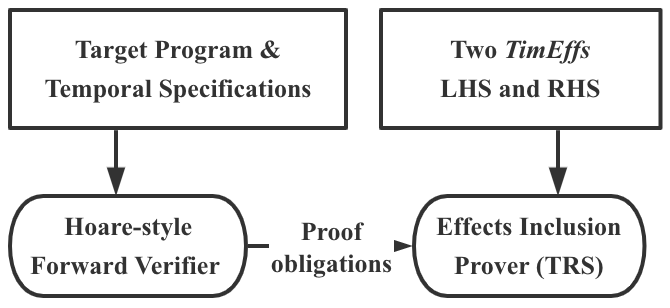
\includegraphics[width=0.5\columnwidth]{verification.png}
        \vspace{-3mm}
\caption{\label{fig:Verification_oberview}System Overview.}
      \vspace{-1mm}
\end{wrapfigure}

An overview of our automated verification system is given in \figref{fig:Verification_oberview} It consists of a Hoare-style forward verifier and a TRS. 
The inputs of the forward verifier are HipHop.js programs annotated with temporal specifications written in \timedEffects (cf. \figref{fig:overview_eg1}). 

The input of the TRS is a pair of effects LHS and RHS, referring to the inclusion LHS \code{\CONTAIN} RHS to be checked 
\textit{(LHS refers to left-hand side effects, and RHS refers to right-hand side effects.)}. Besides, the verifier calls the TRS to prove produced inclusions, i.e., between the effects states and pre/post conditions or assertions (cf. \figref{fig:forward_example}). The TRS will be explained in \secref{sec:Entailment_Prover}. 




In this section, we give an axiomatic semantics model\footnote{Based on the operational semantics of Esterel and JavaScript's asynchrony formally defined in \cite{berry1992esterel} and  \cite{madsen2017model} respectively.} for the core language \code{\timedL}, by formalising a set of forward inductive rules. 
These rules transfer program states and systematically accumulate the effects syntactically. 
To define the model, we introduce an environment \env\ and describe a program state in a four-elements tuple \code{\langle \Pi, H, C, T \rangle}, with the following concrete domains:
\begin{flalign*}
\Pi {\defeq} t {\rightarrow} \pi, \qquad
H  {\defeq} es, \qquad
C {\defeq} \overrightarrow{\textbf{S} {\rightarrow} \Delta}\  | \ \textbf{S}?, \qquad
T {\defeq} t, \qquad 
\env {\defeq} \overrightarrow{\textbf{S}}, \qquad
\Delta {\defeq} \m{Present} \ | \ \m{Absent}  \ | \  \m{Undef}
\end{flalign*}

Let \code{\Pi} represents the pure constraints for all the terms; \code{H} represents the trace of \emph{history}; \code{C} represents the \emph{current} time instance or a waiting signal; 
\code{T} is a term binding \code{C}; 
\env\ be the environment containing all the local and output signals; 
\code{\Delta} marks the signal status. 



%We describe the input and output histories of ESTEREL programs by streams carrying sets of signals.

%which is used for the description of a reactive program. 

%The main difficulty in giving a semantics to \code{\timedL} consists in the idea of instantaneous reactions of ESTEREL programs to input signals. 

%We base this semantics on a functional model of behaviour. We describe the input and output histories of ESTEREL programs by streams carrying sets of signals.


%we mainly present the forward verifier
% based on the syntax of each statement. 

%We present the intermediate representation of program states in \figref{fig:intermediate_representation}




%\noindent   the second element represents the  containing the path constraints (\code{\pi}) and signal assignments (\code{\phi})\footnote{The difference between \code{\textbf{S} = \theta} and \code{\textbf{S} \mapsto \theta } is: the former one denotes the constraints along the execution path, which creates \emph{false} if there are two different status assignments to the same signal; while the latter one records the current status of one signal, and will be overwritten when the presence of a signal had been determined.}; 




\subsection{Forward Inference Rules}
\label{Forward_Rules}

     




\section{Temporal Verification via a TRS}
\label{sec:Entailment_Prover}


The TRS  is an automated entailment checker to prove language inclusions among \timedEffects (cf. \defref{Inclusion} and \tabref{tab:rewriting_tree_send}). It is triggered i) prior to temporal property assertions; ii) prior to module calls for the precondition checking; and iii) at the end of verifying a module for the post condition checking. Given two effects \code{\effect_1,\ \effect_2}, TRS decides if the inclusion \code{\effect_1 \CONTAIN  \effect_2 } is valid. 

During the effects rewriting process, the inclusions are in the form of \code{\Gamma \vdash  \effect_1 \CONTAIN^{\effect}  \effect_2 }, a shorthand for: \code{\Gamma \vdash  \effect \cdot \effect_1 \CONTAIN   \effect \cdot  \effect_2}. To prove such inclusions is to check whether all the possible timed traces in the antecedent \code{\effect_1} are legitimately allowed  in the possible timed traces from the consequent \code{\effect_2}.
\code{\Gamma} is the proof context, i.e., a set of effects inclusion hypothesis, \code{\effect} is the history effects from the antecedent that have been used to match the effects from the consequent.
Note that \code{\Gamma}, \code{\effect} are derived during the inclusion proof. 
The inclusion checking is initially invoked with \code{\Gamma{=}\_} and \code{\effect{=} True : \empt}. 







\paragraph{\textbf{Effects Disjunctions.}}
An inclusion with a disjunctive antecedent succeeds if both disjunctions entail the consequent.  An inclusion with a disjunctive consequent succeeds if the antecedent entails either of the disjunctions.  
{ 
 \begin{gather*}
\frac{ \begin{matrix}
    \text{\code{\Gamma \vdash  \effect_1 \CONTAIN  \effect  \qquad \Gamma \vdash \effect_2 \CONTAIN  \effect}}
  \end{matrix}}{\Gamma \vdash  \effect_1 \vee \effect_2 \CONTAIN  \effect}\  \code{[LHS\text{-}OR]}
\qquad
\frac{ \begin{matrix}
    \text{\code{\Gamma \vdash  \effect \CONTAIN  \effect_1  \quad or \quad \Gamma \vdash \effect \CONTAIN  \effect_2}}
  \end{matrix}}{\Gamma \vdash    \effect \CONTAIN \effect_1 \vee \effect_2}\  \code{[RHS\text{-}OR]}
\end{gather*}



}

Now, the inclusions are disjunction-free formulas. 
Next we provide the definitions and implementations of auxiliary functions \emph{Nullable}(\code{\delta}), \emph{First}(\code{fst}) and \emph{Derivative}(\code{D}) respectively.
Intuitively, the Nullable function \code{\delta(\es)} returns a boolean value indicating whether \code{\es} contains the empty trace; the First function \code{fst_{\pure{\pi}}( \es)} computes a set of possible initial time instances of \code{\pure{\pi} : \es}; and the Derivative function \code{D_{I\# t}^{\pure{\pi}}(\es)} computes a next-state effects after eliminating one time instance \code{I} w.r.t. the execution time \code{t} from the current effects \code{\pure{\pi} : \es}. 



%\subsection{closure of clock constrains}
%how to eliminate the unobservable transitions. 
%
%we allow the $\empt$transitions without carrying constraints and resetting clocks at the same time. 




\begin{definition}[Nullable]\label{Nullable}
Given any time sequence \code{\es}, we recursively define \code{\delta(\es)} as:\\
{
\code{\delta(\es) :bool {=}
\begin{cases}
      \code{true} & \code{if\ \empt \in \es}\\
      \code{false} & \code{if\ \empt \notin \es}
    \end{cases} }
    }, where   
{ 
\begin{gather*}
\code{\delta(\bott) {=} false} 
\qquad\quad
\code{\delta(\empt) {=} true} 
\qquad\quad
\code{\delta(I){=} false}   
\qquad\quad
\code{\delta(\textbf{S}?){=} false}   
\qquad\quad\
    \code{\delta(\esn{\es}{\star} ) {=} true}   
\\ 
\code{\delta(\es_1 \seq \es_2) {=} \delta(\es_1) \wedge \delta(\es_2)}
\qquad\qquad
  \code{\delta(\es_1 \choice \es_2) {=} \delta(\es_1) \vee \delta(\es_2)}   
  \qquad\quad
  \code{\delta(\esn{\es}{\omega} ) {=} false}     
  \\
\code{\delta(\es_1 || \es_2) {=} \delta(\es_1) \wedge \delta(\es_2)}
\qquad\qquad\quad
 \code{\delta(\es \# t) {=} \delta(\es)}
\end{gather*}}
\end{definition}

To better outline our contribution, we first present the original \emph{First} function used in  Antimirov's rewriting system, denoted using \code{fst^\prime}, defined as follows:

\begin{definition}[Antimirov's First]\label{First1}
Let \code{fst^\prime(\es){:=}\{ I\ |\  (I \cdot \es^\prime) \in \llbracket  \es \rrbracket  \}} be the set of initial instances derivable from  sequence \code{\es}. (\code{\llbracket  \es \rrbracket } represents all the traces contained in \code{\es}.)
{ 
 \begin{gather*} 
\code{fst^\prime( \bott) {=} \_ } \qquad\ 
\code{ fst^\prime(\empt) {=} \_} \qquad\ 
\code{fst^\prime( I) {=} \{ I \} }
 \qquad\ 
\code{fst^\prime(  \es_1 {\vee} \es_2) {=} fst^\prime(  \es_1) \cup fst^\prime(  \es_2)}
\\
{
\code{fst^\prime( \esn{\es}{\star} ) {=} fst^\prime({ \es})} 
\qquad\quad\
\code{fst^\prime(\es_1 {\seq} \es_2) {=} } 
\begin{cases}
      \code{\code{fst^\prime(  \es_1)} \cup \code{fst^\prime(  \es_2)} } \quad & \code{ if\ \delta(\es_1) {=} true}\\
      \code{\code{fst^\prime(  \es_1)}} & \code{  if\ \delta(\es_1) {=} false}
    \end{cases} 
    }
\end{gather*}
}
\end{definition}

As shown, \code{fst^\prime} does not handle 
%the concurrent operator \code{||} nor contains 
any arithmetic constraints, nor 
the real-time bounds constructor \code{\#}. Next, we define the novel  \emph{First} function used in this work, denoted using \code{fst}. 
%but helps to build up our \emph{First} function \code{fst}. 

\begin{definition}[First]\label{First}
Let \code{fst_{\pure{\pi}}(\es){:=}\{ (I,  \pi, t) \ |\  \pi {\wedge} t{\geq}0 : (I\# t) \cdot \es^\prime \in \llbracket  \pi {:} \es \rrbracket \}} be the set of initial time instances derivable from effects \code{\pi {:} \es}. (\code{\llbracket  \pi {:} \es \rrbracket } represents all the time  traces contained in \code{\pi {:} \es}) 
{ 
 \begin{gather*} 
\code{fst_{\pure{\pi}}( \bott) {=} \_ } \qquad\quad
\code{fst_{\pure{\pi}}(\empt) {=} \_ } \qquad\quad
\code{fst_{\pure{\pi}}( I ) {=} \{ (I, \pi {\wedge} t{\geq}0, t) \}  \ (t\ is\ fresh)} 
\qquad\quad
   \code{fst_{\pure{\pi}}(  \es \# t) {=}  fst_{pi}(\es)}
 \\
\code{fst_{\pure{\pi}}( \esn{\es}{\star} ) {=} fst_{\pure{\pi}}({ \es})}
\qquad\quad
\code{fst_{\pure{\pi}}( \esn{\es}{\omega} ) {=} fst_{\pure{\pi}}({ \es})} 
\qquad\quad
\code{fst_{\pure{\pi}}(  \es_1 {\vee} \es_2) {=} fst_{\pure{\pi}}(  \es_1) \cup fst_{\pure{\pi}}(  \es_2)  }  \\
\code{fst_{\pure{\pi}}( \textbf{S}? ) {=} fst_{\pure{\pi}}( \{\textbf{S}\} ) \cup fst_{\pure{\pi}}( \{ \overline{\textbf{S}} \} ) }
    \qquad\qquad\quad
   \code{fst_{\pure{\pi}}(  \es_1 {||} \es_2) {=} unify \ 
    (fst_{\pure{\pi}}(  \es_1)) \  (fst_{\pure{\pi}}(  \es_2))  }  
   \\
{
\code{fst_{\pure{\pi}}(\es_1 {\seq} \es_2) {=} } 
\begin{cases}
      \code{\code{fst_{\pure{\pi}}(  \es_1)} \cup \code{fst_{\pure{\pi}}(  \es_2)} } & \code{ if\ \delta(\es_1) {=} true}\\
      \code{\code{fst_{\pure{\pi}}(  \es_1)}} & \code{  if\ \delta(\es_1) {=} false}
    \end{cases} 
    }  
\end{gather*}
}
\end{definition}


\begin{definition}[First-Tuples Unification]\label{unify} Given two first tuples \code{(I_1, \pi_1, t_1)} and \code{(I_2, \pi_2, t_2) }, we define that: 
%We deploy a \code{unify} function to merge two time instances, where \\ 
\code{unify\ (I_1, \pi_1, t_1)\  (I_2, \pi_2, t_2) = (I_1 \cup I_2, \pi_1 \wedge \pi_2 \wedge (t1 {=} t2), t_1)}.
\end{definition}


\begin{definition}[Instances Subsumption]\label{Subsumption}
Given two instances \code{I} and \code{J}, we define the subset relation \code{I {\subseteq} J} as: the set of present signals in \code{J} is a subset of the set of present signals in \code{I}, and the set of absent signals in \code{J} is a subset of the set of absent signals in \code{I}\footnote{As in having more constraints refers to a smaller set of satisfying instances.}.
Formally, 
 \begin{gather*} 
 \code{I {\subseteq} J \Leftrightarrow  \{\textbf{S}\ |\ (\textbf{S} {\mapsto} Present) \in J \}  \subseteq  \{\textbf{S}\ |\ (\textbf{S} {\mapsto} Present) \in I \}} \\
  \code{ \quad\  and  \ 
 \{\textbf{S}\ |\ (\textbf{S} \mapsto Absent) \in J \}  \subseteq  \{\textbf{S}\ |\ (\textbf{S} \mapsto Absent) \in I \}
 }
\end{gather*}

\end{definition}


\begin{definition}[Time Instances Subsumption]\label{Subsumption1}
Given two time instances \code{(I, \pi_1, t_1)} and \code{(J, \pi_2, t_2)}, we define the subset relation \code{(I, \pi_1, t_1) {\subseteq} (J, \pi_2, t_2)} as:  \code{I {\subseteq} J} and \code{\pi_1[t_2/t_1]  {\Rightarrow}   \pi_2  }.

\end{definition}

\begin{definition}[Partial Derivative\footnote{Intuitively, the partial derivative refers to the left quotient of a language equation, for example, for REs, \code{x^{{-}1} \llbracket x\cdot y\rrbracket {=} y};  \code{y^{{-}1} \llbracket x\cdot y\rrbracket {=} \bott}; and  \code{y^{{-}1} \llbracket x + y\rrbracket {=} \epsilon}. Here we come up with a new notion of partial derivative for \timedEffects. 
}]\label{Derivative}
The partial derivative \code{D^{\pi}_{(I, \pi^\prime, t^\prime)}(\es)} 
of effects \code{\pi : \es} 
w.r.t. a time instance \code{(I, \pi^\prime, t^\prime)} computes the  effects for the left quotient \code{(I, \pi^\prime, t^\prime)^{\text{-}1}\llbracket \pi : \es \rrbracket}. \footnote{For understanding of the derivative rule for \code{es\# t} (cf. \tabref{tab:rewriting_tree_send}  step \textcircled{3}), it is essentially splitting \code{\es} with a head and a tail, bound with fresh terms \code{t_1} and \code{t_2} respectively. Meanwhile it unifies \code{t_1} with \code{t^\prime} and  adds the constraint \code{t_1 {+} t_2 {=} t}.}
%\footnote{As the reader may notice, our First and Derivative function does not handle the timed sequences constructed by \code{||}, as the synchronous parallel is reduced during the normalization phase.}
\begin{gather*}
\code{D^{\pi}_{(I, \pi^\prime, t^\prime)}(\bott) {=}}  
 \code{False : \bott} 
\qquad\ 
\code{D^{\pi}_{(I, \pi^\prime, t^\prime)}(  \empt) {=}}   
\code{False : \bott} 
\qquad \ 
\code{D^{\pi}_{(I, \pi^\prime, t^\prime)}(es_1 || es_2)} {=} \code{D^{\pi}_{(I, \pi^\prime, t^\prime)}(es_1)} || \code{D^{\pi}_{(I, \pi^\prime, t^\prime)}( es_2)} 
    \\
        \code{D^{\pi}_{(I, \pi^\prime, t^\prime)}(  \esn{\es}{\star}) } {=} \code{ D^{\pi}_{(I, \pi^\prime, t^\prime)}(  {\es}) \cdot (\esn{\es}{\star})}  
        \qquad\qquad
                \code{D^{\pi}_{(I, \pi^\prime, t^\prime)}(  \esn{\es}{\omega}) } {=} \code{ D^{\pi}_{(I, \pi^\prime, t^\prime)}(  {\es}) \cdot (\esn{\es}{\omega})}  
\\
{
 \code{D^{\pi}_{(I, \pi^\prime, t^\prime)}(   \es_1 \seq \es_2) {=} }
\begin{cases}
      \code{D^{\pi}_{(I, \pi^\prime, t^\prime)}(   \es_1) \cdot  \es_2 \vee  D^{\pi}_{(I, \pi^\prime, t^\prime)}( \es_2)} \quad &\code{if\ \delta(\es_1) {=} true}   \\
      \code{D^{\pi}_{(I, \pi^\prime, t^\prime)}  ( \es_1) \cdot  \es_2} & \code{if\ \delta(\es_1) {=} false} 
    \end{cases} 
    }
 \\
\code{D^{\pi}_{(I, \pi^\prime, t^\prime)}(  \es_1 \choice \es_2) } {=} \code{ D^{\pi}_{(I, \pi^\prime, t^\prime)}(  \es_1) \choice D^{\pi}_{(I, \pi^\prime, t^\prime)}(  \es_2)} 
%\\
%\code{D^{\pi}_{(I, \pi^\prime, t^\prime)}(  \es_1 \ ||\  \es_2) } {=} \code{ D^{\pi}_{(I, \pi^\prime, t^\prime)}(  \es_1) \ ||\ D^{\pi}_{(I, \pi^\prime, t^\prime)}(  \es_2)} 
\\
\code{D^{\pi}_{(I, \pi^\prime, t^\prime)}(  \es \# t) } {=}
\code{
\pi \wedge(t_1{+} t_2 {=}t) \wedge (t_1{=}t^\prime) : (D^{\pi}_{(I, \pi^\prime, t^\prime)}(\es))\# t_2} \ \ \ 
\code{(fresh \ t_1\ t_2 )}
\\
\code{D^{\pi}_{(I, \pi^\prime, t^\prime)}(\textbf{S}?)} {=} \code{\pi: \empt\ (}\code{ I {\subseteq} \{\textbf{S}\})}
\qquad
\code{D^{\pi}_{(I, \pi^\prime, t^\prime)}(\textbf{S}?)} {=} \code{\pi: \textbf{S}?\ (}\code{ I {\not\subseteq} \{\textbf{S}\})}
\\
\code{D^{\pi}_{(I, \pi^\prime, t^\prime)}(J)} {=} \code{\pi: \empt\ (}\code{ I {\subseteq} J)}
\qquad\ 
    \code{D^{\pi}_{(I, \pi^\prime, t^\prime)}( J)} {=} \code{False : \bott \ (}\code{I {\not\subseteq} J)} 
\end{gather*}
\end{definition}




\subsection{Rewriting Rules}
\label{InferenceRules}
Given the well-defined auxiliary functions above, we now discuss the key steps and related rewriting rules that we may use in such an effects inclusion proof.  


\begin{enumerate}
\item 
\textbf{Axiom rules.}
\label{Base}
Analogous to  the standard propositional logic, \code{\bott} (referring to \textit{false}) entails any effects, while no \textit{non-false} effects entails \code{\bott}.
 \begin{gather*}
  \codeme{\frac{
\begin{matrix}
\end{matrix}
}{\text{\code{ \Gamma  \vdash \pi : \bott   \CONTAIN \effect }}}\ [Bot\text{-}LHS]}
\qquad\qquad\quad
\codeme{\frac{
\begin{matrix}
\effect \neq  \pi : \bott 
\end{matrix}
}{\text{\code{\Gamma  \vdash  \effect \not\CONTAIN  \pi : \bott }}} \ \codeme{  [Bot\text{-}RHS]} }
\end{gather*}

\item 
\textbf{Disprove (Heuristic Refutation).}
\label{Refutation}
This rule is used to disprove the inclusions when the antecedent is nullable, while the consequent is not nullable. Intuitively, the antecedent contains at least one more trace (the empty trace) than the consequent. Therefore, the inclusion is invalid. 

\vspace{-4mm}
 \begin{gather*}
\frac{
\begin{matrix}
\text{\codeme{\delta(\es_1) \wedge \neg \delta(\es_2) }}
\end{matrix}
}{\text{\code{\Gamma  \vdash  \pi_1 : \es_1 \not\CONTAIN  \pi_2 : \es_2 }}}\ \codeme{  [DISPROVE]} 
\qquad\ \ 
\frac{
\begin{matrix}
\text{\code{\pi_1 \Rightarrow \pi_2 \quad\ \  
\m{fst}_{\pi_1}(\es_1) = \{\}
%\es_1 \subseteq \es_2 
}}
\end{matrix}
}{\text{\code{\Gamma   \vdash  \pi_1 : \es_1 \CONTAIN  \pi_2 : \es_2 }}}\ \codeme{  [PROVE]} 
\end{gather*}

\item 
\textbf{Prove.}
\label{Prove}
We use two rules to prove an inclusion: (i) \codeme{[PROVE]} is used when the fst set of the antecedent is empty; and (ii) $\code{[REOCCUR]}$ to prove an inclusion
when there exist inclusion hypotheses 
in the proof context $\m{\Gamma}$, which are able to soundly prove the current goal. One of the special cases of this rule is when the identical inclusion is shown in the proof context, we then terminate the procedure and prove it as a valid inclusion. 
 \begin{gather*}
\frac{
\begin{matrix}
\text{\codeme{ (\pi_1 : \es_1 \CONTAIN \pi_3 : \es_3) \in \Gamma  }} 
\quad\ \ 
\text{\codeme{(\pi_3 : \es_3 \CONTAIN  \pi_4 : \es_4) \in {\Gamma} }} \quad\  \ 
\text{\codeme{ (\pi_4 : \es_4 \CONTAIN \pi_2 : \es_2) \in {\Gamma}  }}
\end{matrix}
}{\text{\code{\Gamma  \vdash  \pi_1 : \es_1 \CONTAIN  \pi_2 : \es_2 }} }
\ \codeme{[REOCCUR]}
\end{gather*}

\item 
\textbf{Unfolding (Induction).}
\label{unfolding}
This is the inductive step of unfolding the inclusions. Firstly, we make use of the auxiliary function \code{fst} to get a set of instances \code{F}, which are all the possible initial time instances from the antecedent. 
Secondly, we obtain a new proof context \code{\Gamma^\prime} by adding the current inclusion, as an inductive hypothesis, into the current proof context \code{\Gamma}. 
%(The soundness condition is guaranteed by rule \code{[REOCCUR]} to avoid the possible cyclicity evident in the proof context) 
Thirdly, we iterate each element \code{(I, \pi, t) \in F}, and compute the partial derivatives (\emph{next-state} effects) of both the antecedent and consequent w.r.t \code{(I, \pi, t)}. The proof of the original inclusion succeeds if all the derivative inclusions succeeds.
\begin{gather*}
\frac{ \begin{matrix}
\text{\codeme{F = \m{fst}_{\pure{\pi_1}}(\es_1)\qquad\qquad \Gamma^\prime = \Gamma,  (
\pure{\pi_1} : \es_1 \CONTAIN \pure{\pi_2} : \es_2
)} }\\
    \text{\codeme{\forall (I, \pi, t)\in F. \   (\Gamma^\prime  \vdash \   D_{(I, \pi, t)}^{\pure{\pi_1}}( \es_1) \CONTAIN    D_{(I, \pi, t)}^{\pure{\pi_2}}( \es_2) )}}
  \end{matrix}}
   { \text{\codeme{  \Gamma  \vdash \pure{\pi_1} : \es_1 \CONTAIN \pure{\pi_2} : \es_2 }}}\  \codeme{[UNFOLD]} 
\end{gather*}


\item 
\textbf{Normalization.}
We present a set of normalization rules to soundly transfer the timed effects into a normal form, in particular after getting their derivatives. 
Before getting into the above inference rules, we assume that the effects formulae are tailored accordingly based on the axioms shown in
\tabref{table:normalization}
We built the axiom system on top of a complete axiom system \code{F_1}, from (A1) to (A11), suggested by \cite{salomaa1966two}, which was designed for regular languages. We develop axioms (A12) to (A22) to further accommodate effects constructed by \code{||},   \code{\#} and \code{\omega}.



%\begin{table}[ht]
%\vspace{0mm}
%  \caption{Some Normalization Lemmas for \timedEffects.}
%  \label{table:normalization}
%\setlength{\tabcolsep}{13pt}
%\renewcommand{\arraystretch}{1.1}
%\centering
%\vspace{0mm}
%\begin{tabular}{l || l || l}
%\hline
%  \code{\es \choice \es \rightarrow \es} 
%  &\code{\bott \cdot \es \rightarrow \bott }  
%  &
% 
%  
%\\ \hline
%
%  \code{\bott \choice \es \rightarrow \es } & \code{ \es  \cdot \bott \rightarrow \bott }  &
%
%\code{ (\es_1 \cdot \es_2) \cdot \es_3 \rightarrow \es_1 \cdot (\es_2 \cdot \es_3)}
%\\ \hline
%
%\code{ \es \choice \bott \rightarrow \es }
%&\code{\bott ^\star \rightarrow \empt}
%& 
%
%
%
%\\ \hline
%
%
% \code{\empt \cdot \es  \rightarrow \es }
% &  \code{\epsilon^\star \rightarrow \epsilon}
% &  
%
% 
%\\ \hline
%
%
%\code{ \es \cdot \empt \rightarrow \es}
%& \code{(\empt \vee \es)^\star \rightarrow \es^\star}
%& \code{ }
%
% 
% 
%\\ \hline
%
%
% 
%
%\\ \hline
%
%\end{tabular}
%\vspace{0mm}
%\end{table}

\begin{table}[ht]
\caption{Normalization Axioms for \timedEffects.}
\label{table:normalization}
\setlength{\tabcolsep}{10pt}
\renewcommand{\arraystretch}{1.2}
\centering
\begin{tabular}{rl}
\footnotesize

\begin{minipage}[t]{0.4\textwidth}
\begin{tabular}{||l|l}
\hline
(A1)  &
\code{\es_1 \vee (\es_2 \vee \es_3) \rightarrow   (\es_1 \vee \es_2) \vee \es_3 }\\
\hline
(A2)  &
\code{\es_1 \cdot (\es_2 \cdot \es_3)\rightarrow     (\es_1 \cdot \es_2) \cdot \es_3 }\\
\hline
(A3)  &
\code{\es_1 \vee \es_2 \rightarrow   \es_2 \vee \es_1 }\\
\hline
(A4)  &
\code{\es \cdot (\es_1 \vee \es_2)  \rightarrow \es \cdot \es_1  \vee \es \cdot \es_2 }\\
\hline
(A5)  &
 \code{(\es_1 \vee \es_2)\cdot \es   \rightarrow \es_1 \cdot \es   \vee  \es_2 \cdot \es}\\
\hline
(A6)  &
 \code{\es \vee \es   \rightarrow \es}\\
\hline
(A7)  &
 \code{  \es \cdot \epsilon   \rightarrow \es}\\
\hline
(A8)  &
 \code{  \es \cdot  \bot \rightarrow \bot}\\
\hline
(A9)  &
 \code{\es \vee \bot   \rightarrow \es}\\
\hline
(A10)  &
 \code{\epsilon \vee (\es \cdot \es^\star)   \rightarrow  \es^\star}\\
\hline
(A11)  &
 \code{(\epsilon \vee \es)^\star   \rightarrow  \es^\star}\\
\hline



\end{tabular}
  \end{minipage} 
 
  &
\footnotesize
  \begin{minipage}[t]{0.6\textwidth}
\begin{tabular}{||l|l|}
\hline
(A12)  &
\code{\bot^\omega  \rightarrow \bot }\\
\hline
(A13)  &
\code{\es^\omega \cdot \es_1 \rightarrow \es^\omega }\\
\hline
(A14)  &
\code{\epsilon^\omega \rightarrow \bot }\\
\hline
(A15)  &
\code{ \es\ ||\ \empt \rightarrow \es}\\
\hline
(A16)  &
\code{ \es\ ||\ \bott \rightarrow \bott}\\
\hline
(A17)  &
 \code{(I\# t) \cdot \es_1\ ||\ J \cdot\es_2 \rightarrow ((I  {\cup} J) \# t) \cdot (\es_1 || \es_2)}\\
\hline
(A18)  &
\code{\pi : (\es \# t_1 ) \# t_2 \rightarrow \pi  \wedge (t_1 {=} t_2) : \es \# t_1 }\\
\hline
(A19)  &
 \code{\empt \# t \rightarrow \empt}\\
\hline
(A20)  &
 \code{\bot \# t \rightarrow  \bott}\\
\hline
(A21)  &
 \code{{\pure{False}} : \es \rightarrow {\pure{False}} : \bott}\\
\hline
(A22)  &
 \code{{\pi} : \bott \rightarrow {\pure{False}} : \bott}\\
\hline
 %\code{\es \choice \es \rightarrow \es} 
%  &\code{\bott \cdot \es \rightarrow \bott }  
%  &


\end{tabular}
  \end{minipage}
  

 
\end{tabular}
\end{table}



\end{enumerate}






 
\begin{theorem}[Termination]\label{termination}
The rewriting system TRS is terminating.
\end{theorem}
\begin{proof}
See %the technical report\cite{TR}. 
\appref{proof:TerminationProof}.
\end{proof}

 \begin{theorem}[Soundness]\label{Cyclicsoundness}
Given an inclusion \code{\effect_1 \CONTAIN \effect_2}, if the TRS returns \code{TRUE} when proving \code{\effect_1 \CONTAIN \effect_2}, i.e., it has a cyclic proof, 
then \code{\effect_1 \CONTAIN \effect_2} is valid.
\end{theorem}


\begin{proof}
See %the technical report\cite{TR}. 
\appref{proof:SoundnessProof}.
\end{proof}


%\begin{lemma}
%The set of axioms (A1)-(A11) and (A15)-(A22) are complete for timed effects.
%\begin{proof} 
%
%\end{proof}
%\end{lemma}


 \begin{theorem}[Completeness]\label{Completeness}
 The set of axioms (A1)-(A22) is complete for \timedEffects.

%Given an inclusion \code{\effect_1 \CONTAIN \effect_2}, if \code{\effect_1 \CONTAIN \effect_2} is valid, then the TRS returns  \code{TRUE} by providing a proof.

\end{theorem}

\begin{proof} 
One can observe that by succinct applications of (A17) to (A22), we have a normal form, 
\begin{align}
\pi_1 : (I\# t_1) \cdot \es_1\ ||\ \pi_2 :  (J\# t_2) \cdot\es_2 \rightarrow  (\pi_1 \wedge \pi_2 \wedge t_1{=}t_2) :  ((I  {\cup} J) \# t_1) \cdot (\es_1\ ||\ \es_2)
\end{align}

Then for any ground \timedEffects \code{\es}, the expression \code{\epsilon || \es} can be reduced to either \code{\epsilon} or \code{\es} by the applications of (A15) and (A16).  
The expression \code{\es^\omega} can be reduced to either \code{\bot} or \code{\es^\omega} by the applications of (A12) to (A14).  

Then, by the semantics defined in \figref{fig:Sementic}, effects constructed by Kleene star \code{\star} (possibly finite and possibly infinite) are supersets of effects constructed by \code{\omega} (definite infinite). 

Then one can apply literally all the constructions of \cite{salomaa1966two} used in the completeness proof of \code{F_1} (A1) to (A11).


\end{proof}




\section{Implementation and Case Study}
\label{sec:Evaluation}

\subsection{Implementation}
To show the feasibility of our approach, we have prototyped our automated verification system 
using OCaml \emph{(A demo page  and source code are available from \cite{CODE})}. 
The proof obligations generated by the verifier are discharged using constraint solver Z3 \citep{de2008z3}. 
We prove termination and correctness of the TRS. We validate the front-end forward verifier for conformance, against two implementations: the Columbia Esterel Compiler (CEC) 
\cite{CEC} and Hiphop.js \cite{HH_im}. 


CEC is an open-source compiler designed for research in both hardware and software generation from the Esterel synchronous language to C or Verilog circuit description. It currently supports a subset of Esterel V5, and provides pure Esterel programs for testing. Hiphop.js's implementation facilitates the design of complex web applications by smoothly integrating Esterel and JavaScript, and provides a bench of programs for testing purposes. 



%The core implementation is less than 3500 LOC, roughly, 1{+} LOC for the verifier, and 2{+} LOC for the TRS. We prove the soundness of the TRS. 
%Next, we show case studies to demonstrate the feasibilities of our \timedEffects comparing to Timed Automata. 

%We summarize the underlying reasons which lead to the improvement: (1)When the transition states of the models are small, the average execution time spent by the T.r.s is even less than the automata construction time, which means it is not necessary to construct the automata when a TRS solves it faster; (2)When the total states become larger, on average, the TRS outperforms automata-based algorithms, due to the significantly reduced search branches provided by the normalization lemmas; and (3)For the invalid cases, the TRS disproves them earlier without constructing the whole automata.

%\subsubsection{Experimental Setup}~\\

   %   \vspace{-2mm}
   

Based on these two benchmarks, we validate the verifier using 155  programs, varying from 15 lines to 300 lines. We manually annotate temporal specifications in our timed effects, including both succeeded and failed instances (roughly with the a 1:1 ratio). 
Out of the whole test suite, 101 were from the CEC benchmark, 54 were from the Hiphop.js benchmark.  Since async-await was inherited from JavaScript features, it only presents in the 54 hiphop.js programs.
We conduct experiments on a MacBook Pro with a 2.6 GHz Intel Core i7 processor. Given our benchmark, the running time varying from 0 to 500 ms. 

%We claim that the extra expressiveness gained from our logic is the symbolic time-bounds. The timed effects represent not only one exact Timed Automata but also a set of Timed Automata. Together with our back-end inclusion solver, it enables a verification framework for a group of Automata. More specifically, instead of running the model checker many times for one non-deterministic time-bound at each time, we can define arithmetic constraints bounding the time variable. And to test that, we cover a number of test cases with function calls, and the callee's parameters would be used as the time bounds.

Our implementation is the first that solves the  inclusion problem of symbolic Timed Automata, which is considered important because it overcomes the following main limitations in traditional timed model checking:  i) they cannot be used to specify and verify systems incompletely specified (i. e., whose timing constants are not known yet), and hence cannot be used in early design phases; ii) verifying a system for a set of timing constants usually requires to enumerate all of them one by one if they are supposed to be integer-valued; in addition, Timed Automata cannot be used to verify a system for a set of timing constants that are to be taken in a real-valued dense interval. 



A term rewriting system is efficient because \emph{it only constructs automata as far as it needed}, which makes it more efficient when disproving incorrect specifications, as we can disprove it earlier without constructing the whole automata. In other words, the more incorrect specifications are, the more efficient our solver is.

%
%\subsubsection{Experimental Results}~\\
%\label{subsec:Experimental_Results}
%
%\begin{table}[ht]
%        \vspace{-2mm}
%\caption{\label{tab:Experimental} The experiments are based on 16 real world C programs, we record the lines of code (LOC), the number of testing temporal properties ($\#$Prop.), and the (dis-) proving times (in milliseconds) using PAT and our T.r.s respectively. }
%\centering
%\footnotesize
%\renewcommand{\arraystretch}{1.1}
%\begin{tabular} {l|c|c|c|c}
%\hline
%\textbf{Programs} & \textbf{LOC} & \textbf{$\#$Prop.}  & \textbf{PAT(ms)} & \textbf{T.r.s(ms)} \\ \hline\hline
%1. Chrome\_Dino\_Game    &      80    &    12  &  32.09 &  7.66  \\ \hline
%2. Cradle\_with\_Joystick  &      89     &   12   &  31.22    &   9.85  \\ \hline
%3. Small\_Linear\_Actuator  &    180  &     12  &   21.65      &  38.68  \\ \hline
%4. Large\_Linear\_Actuator &    155   &    12   &  17.41   &   14.66   \\ \hline
%5. Train\_Detect  &                    78   &     12    &   19.50   & 17.35     \\ \hline
%6. Motor\_Control  &                 216  &    15  &     22.89  &  4.71  \\ \hline
%7. Train\_Demo\_2  &                133  &   15    &     49.51   &  59.28   \\ \hline
% 8. Fridge\_Timer  &                  292   &    15   &   17.05   & 9.11 \\ \hline
%  9. Match\_the\_Light   &         143     &    15  &  23.34    &  49.65 \\ \hline
%   10. Tank\_Control  &              104   &    15    &  24.96   &   19.39 \\ 
%     \hline
%  \textbf{\quad \ \ Total}  & 2546    &  235   &  446.88   &   305.33   \\ \hline
%\end{tabular}
%        \vspace{0mm}
%\end{table}
%
%
%        \vspace{-2mm}
%
%
%


\subsection{Case Studies}
\label{subsec:Case_Studies}

Let's recall the existing challenges in different programming paradigms discussed in \secref{sec:Preliminaries}. In this section, we first investigate how our effects logic can help to debug errors related to both synchronous and asynchronous programs. Specifically, it effectively resolves the logical correctness checking (for synchronous languages) and critical anti-patterns checking (for premise asynchrony). 
Meanwhile, we further demonstrate the flexibility and expressiveness of our effects logic. 

%how our proposal makes it flexible for different effects logics.     









\subsubsection{Prove it when Reoccur}~\\

   %   \vspace{-2mm}
%(\code{\{Go\} \Rightarrow \_})
%(\code{\{Ready\} \Rightarrow \_}, \code{t_L^2 \Rightarrow true})
Termination of TRS is guaranteed because the set of derivatives to be considered is finite, and possible cycles are detected using \emph{memorization} \cite{brotherston2005cyclic}, i.e., the rule \code{[REOCCUR]}. % Check out this following example: 






As shown in \tabref{tab:reoccur}, the LHS formula is a disjunction of two effects. An inclusion with a disjunctive antecedent succeeds if both disjunctions entail the consequent, shown in step \code{\textcircled{1}}.  
%Now we have 2 subtrees, the first subtree is for
%  \code{
%    \textcolor {darkred}{t_L{<}3} : \{A\}^\star \# t_L \cdot \{B\}
%    \CONTAIN
%    \textcolor {darkred}{t_R{<}4} : \{A\}^\star \# t_R \cdot \{B\}
%  }
%and the second one is for
%  \code{
%    \textcolor {darkred}{True} : {B} \CONTAIN
%    \textcolor {darkred}{t_R{<}4} : \{A\}^\star \# t_R \cdot \{B\}
%  }.
%In order to prove the original proposition, both of the two new propositions have
%to be proved.
%Using the disjunction rule \code{\effect_1 \vee \effect_2 \CONTAIN \effect \iff
%\effect_1 \CONTAIN \effect \ and \  \effect_2 \CONTAIN \effect}, we split the proposition
%in . 
In step \code{\textcircled{2}} of the first sub-tree, in order to eliminate the first instance \code{\{B\}}, \code{\{A\}^\star \# t_R} has to be reduced to be \code{\epsilon}, therefore the time constraints have nothing to do in this branch. 
% is 
%eliminated by \code{\epsilon}, 
Then in steps \code{\code{\textcircled{4}}}, we
can simply prove it with the side constraint entailment \code{\textcolor {darkred}{True} \Rightarrow  \textcolor {darkred}{True}} succeed.
%and \code{\epsilon \CONTAIN \epsilon}. 


Looking at the second sub-tree, in step \code{\textcircled{5}}, \code{t_L} and \code{t_R} are firstly split 
into \code{t_L^1{+}t_L^2} and \code{t_R^1{+}t_R^2}. 
Then in step \code{\textcircled{6}}, 
\code{\{A\} \# t_L^1} together with \code{\{A\} \# t_R^1} are eliminated, unifying \code{t_L^1} and \code{t_R^1} (adding the constraint \code{ t_L^1 {=}  t_R^1}).
%, also
%are unified as new constraint \code{t_L^1{=}t_R^1}.
In step \code{\textcircled{7}}, we observe the proposition is isomorphic with one of the the previous step, marked using \code{\textcolor{darklavender}{(\ddagger)}}. 
%one in
%step \code{\textcircled{1}}, 
Hence we apply the rule \code{[REOCCUR]} to prove it with a succeed side constraints entailment: \code{\textcolor {
      darkred}{t_L^1{+}t_L^2{=}t_L \wedge t_L{<}3 \wedge t_R{=}t_R^1{+}t_R^2 \wedge t_L^1{=}t_R^1
      \wedge t_L^2{=}t_R^2
    }\Rightarrow
    \textcolor {darkred}{t_R{<}4} }. 
%Since the structure of terms \code{t_L^2, t_L} and \code{t_R^2, t_R} are isomorphic,
%we will need to unify \code{t_L^2} and \code{t_R^2} in order to get enough
%time constraints. And in step \code{\textcircled{5}} we prove the proposition to
%be true.


{
\begin{table}[ht]
      \vspace{0mm}
\caption{\label{tab:reoccur} The reoccurrence proving example. 
\code{I:} The main rewriting proof tree; \code{II:} Right hand side sub-tree of the rewriting process.}
      
\vspace{-1mm}
\begin{adjustbox}{width=1\textwidth}
 \Large\begin{tabular}[t]{l}
  \hline\\
 

\code{I:}\
{

\begin{prooftree}


\Hypo{
  \code{
    \textcolor {darkred}{True} \Rightarrow  \textcolor {darkred}{True} \qquad
    \epsilon \CONTAIN \epsilon
  }
}

\Infer[dashed]1[{\siderule{\textcircled{4}[PROVE]}}]{
  \code{
    \textcolor {darkred}{True} : \epsilon \CONTAIN
    \textcolor {darkred}{True} : \epsilon
  }
}

\Infer[dashed]1[{\siderule{\textcircled{3}[Normalisation]}}]{
  \code{
    \textcolor {darkred}{True} : \cancel{\{B\}} \CONTAIN
    \textcolor {darkred}{True} : \cancel{\empt \cdot \{B\}}
  }
}

\Infer[dashed]1[{\siderule{\textcircled{2}[UNFOLD]}}]{
  \code{
    \textcolor {darkred}{True} : \{B\} \CONTAIN
    \textcolor {darkred}{t_R{<}4} : \{A\}^\star \# t_R \cdot \{B\}
  }
}
\Hypo{\code{II}}

\Infer[dashed]1[{\siderule{}}]{
  \code{
    \textcolor {darkred}{t_L{<}3} {:} \{A\}^\star \# t_L {\cdot} \{B\}
    \CONTAIN
    \textcolor {darkred}{t_R{<}4} {:} \{A\}^\star \# t_R {\cdot} \{B\}
  }
}

\Infer[dashed]2[{\siderule{\textcircled{1}[Disj\text{-}L]}}]{
  \code{
    \textcolor {darkred}{t_L{<}3} : \{A\}^\star \# t_L \cdot \{B\}
    \vee \textcolor {darkred}{True} : \{B\} \CONTAIN
    \textcolor {darkred}{t_R{<}4} : \{A\}^\star \# t_R \cdot \{B\}
  }
}
\end{prooftree}}
\\~\\ 

\hline \\
\code{II:} 
{\begin{prooftree}
\Hypo{
  \code{
    \textcolor {
      darkred}{t_L^1{+}t_L^2{=}t_L \wedge t_L{<}3 \wedge t_R{=}t_R^1{+}t_R^2 \wedge t_L^1{=}t_R^1
      \wedge t_L^2{=}t_R^2
    } \Rightarrow
    \textcolor {darkred}{t_R{<}4} 
%\qquad
%     \{A\}^\star \cdot \{B\}
%    \CONTAIN
%     \{A\}^\star \cdot \{B\}
  }
}

\Infer[dashed]1[{\siderule{}}]{
  \code{
    \textcolor {
      darkred}{\cdots {\wedge} \cdots
%      
%      t_L^1{+}t_L^2{=}t_L{<}3 {\wedge} t_R{=}t_R^1{+}t_R^2 {\wedge} t_L^1{=}t_R^1
%      {\wedge} t_L^2{=}t_R^2
    } :
     \{A\}^\star \# t_L^2 \cdot \{B\}
    \CONTAIN
    \textcolor {darkred}{t_R{<}4} :
     \{A\}^\star \# t_R^2 \cdot \{B\} \quad  \textcolor{darklavender}{(\ddagger)}
  }
}

\Infer[dashed]1[{\siderule{\textcircled{7}[REOCCUR]}}]{
  \code{
    \textcolor {
      darkred}{
%t_L^1{+}t_L^2{=}t_L {\wedge} t_R{=}t_R^1{+}t_R^2 {\wedge}      
       t_L^1{=}t_R^1
    } :
     \cancel{\{A\} \# t_L^1} {\cdot} \{A\}^\star \# t_L^2 \cdot \{B\}
    \CONTAIN
    \textcolor {darkred}{t_R{<}4} :
     \cancel{\{A\} \# t_R^1} {\cdot} \{A\}^\star \# t_R^2 \cdot \{B\}
  }
}

\Infer[dashed]1[{\siderule{\textcircled{6}[UNFOLD]}}]{
  \code{
    \textcolor {darkred}{t_L^1{+}t_L^2{=}t_L {\wedge} t_R{=}t_R^1{+}t_R^2} :
     ( \{A\} \# t_L^1 {\cdot} \{A\}^\star \# t_L^2) \cdot \{B\}
    \CONTAIN
    \textcolor {darkred}{t_R{<}4} :
     ( \{A\} \# t_R^1 {\cdot} \{A\}^\star \# t_R^2) \cdot \{B\}
  }
}

\Infer[dashed]1[{\siderule{\textcircled{5}[SPLIT]}}]{
  \code{
    \textcolor {darkred}{t_L{<}3} : \{A\}^\star \# t_L \cdot \{B\}
    \CONTAIN
    \textcolor {darkred}{t_R{<}4} : \{A\}^\star \# t_R \cdot \{B\}  \quad \textcolor{darklavender}{(\ddagger)}
  }
}
\end{prooftree}}

\\~\\

\hline
    
\end{tabular}
\end{adjustbox}
            \vspace{-3mm}
\end{table}
}



\subsection{Discussion}

As the examples show, our proposed effects logic and the abstract semantics for \code{\timedL} not only tightly capture the behaviours of a mixed synchronous and asynchronous concurrency model but also help to mitigate the programming challenges in each paradigm. Meanwhile, the inferred temporal traces from a given reactive program enable a compositional timed temporal verification at the source level, which is not yet supported by existing temporal verification techniques. 






\section{Related Work}\label{sec:Related_work}





\subsection{Specifications and Real-Time Verification}





%Formally, given a KA is \code{(A,+,\cdot, \star,  0, 1)}, a SKA over a finite set \code{A_B} is \code{(A,+, \cdot, \times, \star,  0, 1,  A_B)}, \code{A_B {\subseteq} A}. 
%Our \code{\bot} corresponds to the \code{0}; our \code{\empt} corresponds to the \code{1}; our \emph{time instance} containing simultaneous signals can be expressed via \code{\times}; 

Compositional specification for real-time systems based on timed process algebras has been extensively studied. Examples include the CCS\code{\text{+}}Time \cite{yi1991ccs} and Timed CSP \cite{dong2008timed}.  
The differences are: 
i) in CCS\code{\text{+}}Time, if there is no timed constraints specified, transitions takes no time; whereas in our effects logic, it means \code{true} (arbitrary time), which is more close to the real life context where the time bounds are often unpredictable.
ii) Timed CSP does not allow explicit representation of real-time through the manipulation of clock variables.

%relies on implicit clocks, which means it 


There have been a number of translation-based approaches on building verification support for timed process algebras. For example, Timed CSP \cite{dong2008timed} is translated to Timed Automata (TA) so that the model checker Uppaal can be \cite{DBLP:journals/sttt/LarsenPY97} applied. 
TA are finite state automata equipped with clock variables. Models based on TA often have simple structures. For example, the input models of the Uppaal are networks of TA with no hierarchy. 

%Given the well-established TA techniques, 

In practice, system requirements are often structured into phases, which are then composed in many different ways, while TA is deficiency in modelling complex compositional systems. Users often need to manually cast high-level requirements into a set of clock variables with carefully calculated clock constraints, which is tedious and error-prone \cite{sun2013modeling}. 
%Also real-time system modelling based on timed process algebras often suffers from lack of language features or automated tool support. 
On the other hand, all the translation-based approaches share the common problem: 
%i) the worst-case complexity of any efficient  equivalences/inclusion checking algorithm \cite{de2006antichains} %based on such translation 
%goes  exponential in the number of automata states; and ii) 
the overhead introduced by
the complex translation makes it particularly inefficient when \emph{disproving} properties. 

We believe in that the goal of verifying real-time systems, in particular safety-critical systems is to check logical temporal properties, which can be done without constructing the whole reachability graph or the full power of model-checking. We are of the opinion that our approach is simpler as it is based directly on constraint-solving techniques and can be fairly efficient in verifying systems consisting of many components as it avoids to explore the whole state-space \cite{song2020automated,yi1995automatic}.

%About that, between TRS and the construction of efficient automata, recent work \cite{song2020automated} has shown that the former has a minor performance advantage (over a
%benchmark suite) when it is compared with
%state-of-the-art PAT \cite{sun2009pat} model checker.
%Improvement came from the avoidance of the more
%expensive automata construction process.

Moreover, our \timedEffects also draws similarities to Synchronous Kleene Algebra (SKA) \cite{prisacariu2010synchronous}. 
%Antimirov and Mosses' algorithm \cite{antimirov1995rewriting} was designed for deciding the inclusion of regular expressions.   
Kleene algebra (KA) is a decades-old sound and complete equational theory of regular expressions. Among many extensions of KA,
 %timed synchronous 
  SKA is KA extended with a synchrony combinator for actions. In particularly, SKA's \emph{demanding relation} can be reflected by our \emph{instances subsumption} (\defref{Subsumption}), which contributes to the inductive unfolding process. 
Yet our timed effects further capture the time bounds constraints by adding the operator \code{\#}, adapting to real-time system modelling and verification, which is not covered by any existing KA variants/extensions. 



%Presently, SKA allows the synchrony combinator \code{\times} to be expressed over any two SKA terms to support concurrency.
%We achieve a similar outcome in Synced Effects by supporting normalization operations during trace synchronization, via a \code{zip} function in the forward rule of \code{[FV\text{-}Par]}.
%This leads to one major difference in the inclusion/equivalence checking procedure, whereby a TRS for SKA would have to rely on
%\emph{nullable}, \emph{first}, and \emph{partial derivatives} for terms constructed by the added combinator \code{\times}, but
%carefully avoided by our TRS construction. 

While the original equivalence checking algorithm for SKA terms in \cite{prisacariu2010synchronous} has
relied on well-studied decision procedures based on classical Thompson \code{\epsilon}-NFA construction, prior work \cite{broda2015deciding}  shows that the use of Antimirov's partial derivatives
could result in better average-case algorithms for automata construction. 
%Our present work avoided the consideration for the more general \code{\times} operation from SKA
%and customized the TRS for inclusion (instead of equivalence) checking. These decisions led to some opportunities for improvements.
Moreover, between TRS and the construction of efficient automata, prior work has recently shown in \cite{song2020automated} that the former has a minor performance advantage (over a benchmark suite) when it is compared with state-of-the-art PAT \cite{sun2009pat} model checker.
Improvement came from the avoidance of the more expensive automata construction process.



\subsection{Existing Traces-Based Effects Systems} 



Combining program events with a temporal program logic for asserting properties of event traces yields a powerful and general engine for enforcing program properties. Results in \cite{skalka2008types,skalka2004history,marriott2003resource} have demonstrated that static approximations of program event traces can be generated by type and effect analyses \cite{talpin1994type,amtoft1999type}, in a form amenable to existing model-checking techniques for verification. We call these approximations trace-based effects.

Trace-based analyses have been shown capable of statically enforcing flow-sensitive security properties such as safe locking behaviour \cite{foster2002flow} and resource usage policies such as file usage protocols and memory management \cite{marriott2003resource}. In \cite{bartoletti2005enforcing}, a trace effect analysis is used to enforce secure service composition. 
 Stack-based security policies are also amenable to this form of analysis, as shown in \cite{skalka2004history}. 
 

 
 %  has effects capturing sequences of events, including requirements about things that must have happened prior to executing a given block of code

 
More related to our work, prior research has been extending Hoare logic with event traces. The work \cite{malecha2011trace} focuses on finite traces (terminating runs) for web applications, leaving the divergent computation, which indicates \code{false}, verified for every specification. The work \cite{nakata2010hoare} focuses on infinite traces (non-terminating runs) by providing coinductively trace definitions. 
More recent works \cite{bubel2015dynamic,song2020automated} proposed dynamic logics and unified operators to reason about possibly finite and infinite traces at the same time. 

Moreover, this paper draws similarities to \textit{contextual effects} \cite{neamtiu2008contextual}, which computes the effects that have already occurred as the prior effects. The effects of the computation yet to take place as the future effects. 
Besides, prior work \cite{nielson1998behaviour} proposes an annotated type and effect system and infers behaviours from CML \cite{reppy1993concurrent} programs for channel-based communications, though it did not provide any inclusion solving process. 



However, none of the previous works have considered adding real-time abstractions into the modelling for a more extensive timed verification, which is our work's main contribution.
 %The purely algebraic TRS is flexible to accommodate possibly extended expressiveness for the effects logics. Furthermore, as an extension of prior work \cite{song2020automated}, this work is able to reason about both finite and infinite traces, using cyclic proof techniques established  from \cite{brotherston2005cyclic}.




 
%due to the reason that Hoare logic only captures partial correctness, 
%
%
% only captures partial correctness, 
%
%
%deploys a Hoare logics based on  while its  networking library does not capture timeout, making certain properties difficult or impossible to specify. And because 
%
 

%While  , , the reasoning on timed traces is new. Prior timed effects in precondition is also new, allowing greater safety to be applied to sequential reactive controlling systems such as web applications, communication protocols and IoT systems.





%
%
%compare to Timed Automata:
%modular and can plug in anywhere. 
%absolute time and relative time. 
%$
%//
%(lower_t, upper_time)
%lower_ti<=upper_t
%lower_t<5
%lower_t>8
%modular and can plug in anywhere. 
%absolote time and relative time. 
%it can be only for synchronous system, t.sync, 
%or or real time t.rt.dur. 
%$


\section{Conclusion}
\label{sec:conclusion}
%HipHop.js
We define the syntax and semantics of the novel \timedEffects, to capture reactive program behaviours and  temporal properties. We demonstrate how to give a rather axiomatic semantics to \code{\timedL} by timed-trace processing functions. We use this semantic model to enable  a Hoare-style forward verifier,  which computes the program effects constructively.
We present an effects inclusion checker (the TRS) to prove the annotated temporal properties efficiently. We prototype the verification system and show its feasibility.
To the best of our knowledge, our work is the first that formulates semantics of a mixed Sync-Async concurrency paradigm; and that automates modular timed verification for reactive programs using an expressive effects logic. 


%%
%% The acknowledgments section is defined using the "acks" environment
%% (and NOT an unnumbered section). This ensures the proper
%% identification of the section in the article metadata, and the
%% consistent spelling of the heading.
%\begin{acks}
%To Robert, for the bagels and explaining CMYK and color spaces.
%\end{acks}

%%
%% The next two lines define the bibliography style to be used, and
%% the bibliography file.



\bibliographystyle{ACM-Reference-Format}
\bibliography{references}
%% Citation style
%% Note: author/year citations are required for papers published as an
%% issue of PACMPL.


%%
%% If your work has an appendix, this is the place to put it.
\appendix

\section{Termination Proof}  \label{proof:TerminationProof}

\begin{proof}\label{proof:termination} 
Let Set[\inclusion] be a data structure representing the sets of inclusions. 

We use \code{S} to denote the inclusions to be proved, and \code{H} to accumulate  "inductive hypotheses", i.e., \code{S,  H \in Set[\inclusion]}.

Consider the following partial ordering \code{\succ} on pairs \code{\langle S, H \rangle}:
\begin{gather*}
\code{\langle S_1, H_1 \rangle \succ \langle S_2, H_2 \rangle}\ \ \text{iff}\ \ \code{|H_1| < |H_2| \vee 
(|H_1| = |H_2| \wedge |S_1| > |S_2|)}. 
\end{gather*}
where \code{|X|} stands for the cardinality of a set \code{X}.  Let \code{\Rightarrow} donate the rewrite relation, then \code{\Rightarrow^*} denotes its reflexive transitive closure. For any given \code{S_0}, \code{H_0}, this ordering is well founded on the set of pairs \code{\{\langle S, H \rangle | \langle S_0, H_0 \rangle \Rightarrow^* \langle S, H \rangle \}}, due to the fact that \code{H} is a subset of the finite set of pairs of all possible derivatives in initial inclusion.


Inference rules in our TRS given in \secref{InferenceRules} transform current pairs \code{\langle S, H \rangle} to new pairs \code{\langle S^\prime, H^\prime \rangle}. 
And each rule either increases \code{|H|} (Unfolding) or, otherwise, reduces \code{|S|} (Axiom, Disprove, Prove), therefore the system is terminating.




 \end{proof}


\section{Soundness Proof} 
 \label{proof:SoundnessProof}
 

 

\begin{proof}
For each inference rules, if inclusions in their premises are valid, and their side conditions are satisfied, then goal inclusions in their conclusions are valid.

\begin{enumerate}
\item \textbf{Axiom Rules:} 
 \begin{gather*}
  \codeme{\frac{
\begin{matrix}
\end{matrix}
}{\text{\code{ \Gamma  \vdash \pi : \bott   \CONTAIN \effect }}}\ [Bot\text{-}LHS]}
\qquad\qquad\quad
\codeme{\frac{
\begin{matrix}
\effect \neq  \pi : \bott 
\end{matrix}
}{\text{\code{\Gamma  \vdash  \effect \not\CONTAIN  \pi : \bott }}} \ \codeme{  [Bot\text{-}RHS]} }
\end{gather*}
- It is easy to verify that antecedent of goal entailments in the rule \codeme{[Bot\text{-}LHS]} is unsatisfiable. Therefore, these entailments are evidently valid.\\
- It is easy to verify that consequent of goal entailments in the rule \codeme{[Bot\text{-}RHS]} is unsatisfiable. Therefore, these entailments are evidently invalid.\\


\item \textbf{Disprove Rules:} 
 \begin{gather*}
\frac{
\begin{matrix}
\text{\codeme{\delta(\es_1) \wedge \neg \delta(\es_2) }}
\end{matrix}
}{\text{\code{\Gamma  \vdash  \pi_1 : \es_1 \not\CONTAIN  \pi_2 : \es_2 }}}\ \codeme{  [DISPROVE]} 
\qquad\ \ 
\frac{
\begin{matrix}
\text{\code{\pi_1 \Rightarrow \pi_2 \quad\ \  
\m{fst}_{\pi_1}(\es_1) = \{\}
%\es_1 \subseteq \es_2 
}}
\end{matrix}
}{\text{\code{\Gamma   \vdash  \pi_1 : \es_1 \CONTAIN  \pi_2 : \es_2 }}}\ \codeme{  [PROVE]} 
\end{gather*}
- It's straightforward to prove soundness of the rule \codeme{[DISPROVE]}, Given that \codeme{ \es1} is nullable, while \codeme{ \es_2} is not nullable, thus clearly the antecedent contains more event traces than the consequent.  Therefore, these entailments are evidently invalid.\\


\item \textbf{Prove Rules:} 
 \begin{gather*}
\frac{
\begin{matrix}
\text{\codeme{ (\pi_1 : \es_1 \CONTAIN \pi_3 : \es_3) \in \Gamma  }} 
\quad\ \ 
\text{\codeme{(\pi_3 : \es_3 \CONTAIN  \pi_4 : \es_4) \in {\Gamma} }} \quad\  \ 
\text{\codeme{ (\pi_4 : \es_4 \CONTAIN \pi_2 : \es_2) \in {\Gamma}  }}
\end{matrix}
}{\text{\code{\Gamma  \vdash  \pi_1 : \es_1 \CONTAIN  \pi_2 : \es_2 }} }
\ \codeme{[REOCCUR]}
\end{gather*}
- To prove soundness of the rule \code{[PROVE]}, we consider an arbitrary model, \codeme{d,  \varphi} such that:  \codeme{d,  \varphi \models  {\pi_1 : \es_1}}. Given the side conditions from the promises, we get \codeme{d,  \varphi \models {\pi_2 : \es_1}}. When the \code{\m{fst}} set of \code{\es_1} is empty, \code{\es_1} is possible \code{\bot} or \code{\epsilon}; and \code{\es_2} is nullable. For both cases, the inclusion is valid. 

- To prove soundness of the rule \codeme{[REOCCUR]}, we consider an arbitrary model, \codeme{d,  \varphi} such that:  \codeme{d,  \varphi \models  {\pi_1 : \es_1}}. Given the promises that  \codeme{\pi_1 : \es_1 \CONTAIN \pi_3 : \es_3}, we get \codeme{d,  \varphi \models {\pi_3 : \es_3}}; Given the promise that there exists a hypothesis \codeme{\pi_3 : \es_3 \CONTAIN  \pi_4 : \es_4}, we get \codeme{d,  \varphi \models {\pi_4 : \es_4}}; Given the promises that  \codeme{\pi_4 : \es_4 \CONTAIN \pi_2 : \es_2}, we get \codeme{d,  \varphi \models {\pi_2 : \es_2}}. Therefore,  the inclusion is valid. 
\\


\item \textbf{Unfolding Rule:} 
\begin{gather*}
\frac{ \begin{matrix}
\text{\codeme{F = \m{fst}_{\pure{\pi_1}}(\es_1)\qquad\qquad \Gamma^\prime = \Gamma,  (
\pure{\pi_1} : \es_1 \CONTAIN \pure{\pi_2} : \es_2
)} }\\
    \text{\codeme{\forall (I, \pi, t)\in F. \   (\Gamma^\prime  \vdash \   D_{(I, \pi, t)}^{\pure{\pi_1}}( \es_1) \CONTAIN    D_{(I, \pi, t)}^{\pure{\pi_2}}( \es_2) )}}
  \end{matrix}}
   { \text{\codeme{  \Gamma  \vdash \pure{\pi_1} : \es_1 \CONTAIN \pure{\pi_2} : \es_2 }}}\  \codeme{[UNFOLD]} 
\end{gather*}


- To prove soundness of the rule \codeme{[UNFOLD]}, we consider an arbitrary model, \codeme{d_1,  \varphi_1} and \codeme{d_2,  \varphi_2}  such that:  \codeme{d_1,  \varphi_1 \models {\pi_1 : \es_1}} and \codeme{d_2,  \varphi_2 \models  {\pi_2 : \es_2}}. For an arbitrary time instance \codeme{(I, \pi, t)}, let \codeme{d_1^\prime, {\varphi_1}^\prime \models \codeme{(I, \pi, t)}^{\text{-}1}\llbracket  \pi_1: \es_1 \rrbracket}; and 
\codeme{d_2^\prime, {\varphi_2}^\prime \models \codeme{(I, \pi, t)}^{\text{-}1}\llbracket \pi_2 : \es_2 \rrbracket}. 

Case 1), \codeme{\codeme{(I, \pi, t)} \notin F}, \codeme{d_1^\prime, {\varphi_1}^\prime \models \bott}, thus automatically \codeme{d_1^\prime, {\varphi_1}^\prime \models D^{\pi_2}_{\codeme{(I, \pi, t)}}( \es_2)};

Case 2), \codeme{\codeme{(I, \pi, t)} \in F}, given that inclusions in the rule's premise is valid, then \codeme{d_1^\prime, {\varphi_1}^\prime \models D^{\pi_2}_{\codeme{(I, \pi, t)}}( \es_2)}. 

By \defref{Inclusion}, since for all \codeme{(I, \pi, t)}, \codeme{D^{\pi_1}_{\codeme{(I, \pi, t)}} (\es_1) \CONTAIN    D^{\pi_2}_{\codeme{(I, \pi, t)}}( \es_2)}, the conclusion is valid. 
\\

\end{enumerate}
All the inference rules used in the TRS are sound, therefore the TRS is sound.
\end{proof}

% \section{Completeness Proof} 
% \label{proof:Completeness}
 



\end{document}
\endinput
%%
%% End of file `sample-manuscript.tex'.
